\documentclass[10pt,fleqn]{article} % Default font size and left-justified equations
\usepackage[%
    pdftitle={Modélisation systèmes multiphysiques : Modélisation linéaire et non linéaire},
    pdfauthor={Xavier Pessoles}]{hyperref}
    
%%%%%%%%%%%%%%%%%%%%%%%%%%%%%%%%%%%%%%%%%
% Original author:
% Mathias Legrand (legrand.mathias@gmail.com) with modifications by:
% Vel (vel@latextemplates.com)
% License:
% CC BY-NC-SA 3.0 (http://creativecommons.org/licenses/by-nc-sa/3.0/)
%%%%%%%%%%%%%%%%%%%%%%%%%%%%%%%%%%%%%%%%%

%----------------------------------------------------------------------------------------
%	VARIOUS REQUIRED PACKAGES AND CONFIGURATIONS
%----------------------------------------------------------------------------------------

%\usepackage[top=2.5cm,bottom=2cm,left=2cm,right=2cm,headsep=40pt,a4paper]{geometry} % Page margins

\usepackage{graphicx} % Required for including pictures
\graphicspath{{images/}} % Specifies the directory where pictures are stored

\usepackage{lipsum} % Inserts dummy text

\usepackage{tikz} % Required for drawing custom shapes

\usepackage[french]{babel} % English language/hyphenation
\frenchbsetup{StandardLists=true} % Pour éviter la collision babel enumitem pour les listes

\usepackage{enumitem} % Customize lists
\setlist{nolistsep} % Reduce spacing between bullet points and numbered lists

\usepackage{booktabs} % Required for nicer horizontal rules in tables

\usepackage{xcolor} % Required for specifying colors by name
%\definecolor{ocre}{RGB}{243,102,25} % Define the orange color used for highlighting throughout the book
 \definecolor{ocre}{RGB}{49,133,156} % Couleur ''bleue''
\definecolor{violetf}{RGB}{112,48,160} % Couleur ''violet''
\usepackage{enumitem}
\usepackage{pifont} % Pour les dinglist
\usepackage{multicol}
\usepackage{array} % Centrage vertical dans les tableaux

%----------------------------------------------------------------------------------------
%	FONTS
%----------------------------------------------------------------------------------------

\usepackage{avant} % Use the Avantgarde font for headings
%\usepackage{times} % Use the Times font for headings
%\usepackage{mathptmx} % Use the Adobe Times Roman as the default text font together with math symbols from the Sym­bol, Chancery and Com­puter Modern fonts
\usepackage[adobe-utopia]{mathdesign}
\usepackage{microtype} % Slightly tweak font spacing for aesthetics
\usepackage[utf8]{inputenc} % Required for including letters with accents
\usepackage[T1]{fontenc} % Use 8-bit encoding that has 256 glyphs

%----------------------------------------------------------------------------------------
%	BIBLIOGRAPHY AND INDEX
%----------------------------------------------------------------------------------------

%\usepackage[style=alphabetic,citestyle=numeric,sorting=nyt,sortcites=true,autopunct=true,babel=hyphen,hyperref=true,abbreviate=false,backref=true,backend=biber]{biblatex}
%\addbibresource{bibliography.bib} % BibTeX bibliography file
%\defbibheading{bibempty}{}

\usepackage{calc} % For simpler calculation - used for spacing the index letter headings correctly
\usepackage{makeidx} % Required to make an index
\makeindex % Tells LaTeX to create the files required for indexing

%----------------------------------------------------------------------------------------
%	MAIN TABLE OF CONTENTS
%----------------------------------------------------------------------------------------

\usepackage{titletoc} % Required for manipulating the table of contents

\setcounter{tocdepth}{2}     % Dans la table des matieres
\setcounter{secnumdepth}{2}

\contentsmargin{0cm} % Removes the default margin

% Part text styling
\titlecontents{part}[0cm]
{\addvspace{20pt}\centering\large\bfseries}
{}
{}
{}

% Chapter text styling
\titlecontents{chapter}[1.25cm] % Indentation
{\addvspace{12pt}\large\sffamily\bfseries} % Spacing and font options for chapters
{\color{ocre!60}\contentslabel[\Large\thecontentslabel]{1.25cm}\color{ocre}} % Chapter number
{\color{ocre}}  
{\color{ocre!60}\normalsize\;\titlerule*[.5pc]{.}\;\thecontentspage} % Page number

% Section text styling
\titlecontents{section}[1.25cm] % Indentation
{\addvspace{3pt}\sffamily\bfseries} % Spacing and font options for sections
{\color{ocre!60}\contentslabel[\thecontentslabel]{1.25cm} \color{ocre}} % Section number
{\color{ocre}}
{\hfill\color{ocre!60}\thecontentspage} % Page number
[]

% Subsection text styling
\titlecontents{subsection}[1.25cm] % Indentation
{\addvspace{1pt}\sffamily\small} % Spacing and font options for subsections
{\contentslabel[\thecontentslabel]{1.25cm}} % Subsection number
{}
{\ \titlerule*[.5pc]{.}\;\thecontentspage} % Page number
[]


% Subsection text styling
\titlecontents{subsubsection}[1.25cm] % Indentation
{\addvspace{1pt}\sffamily\small} % Spacing and font options for subsections
{\contentslabel[\thecontentslabel]{1.25cm}} % Subsection number
{}
{\ \titlerule*[.5pc]{.}\;\thecontentspage} % Page number
[]

% List of figures
\titlecontents{figure}[0em]
{\addvspace{-5pt}\sffamily}
{\thecontentslabel\hspace*{1em}}
{}
{\ \titlerule*[.5pc]{.}\;\thecontentspage}
[]

% List of tables
\titlecontents{table}[0em]
{\addvspace{-5pt}\sffamily}
{\thecontentslabel\hspace*{1em}}
{}
{\ \titlerule*[.5pc]{.}\;\thecontentspage}
[]

%----------------------------------------------------------------------------------------
%	MINI TABLE OF CONTENTS IN PART HEADS
%----------------------------------------------------------------------------------------

% Chapter text styling
\titlecontents{lchapter}[0em] % Indenting
{\addvspace{15pt}\large\sffamily\bfseries} % Spacing and font options for chapters
{\color{ocre}\contentslabel[\Large\thecontentslabel]{1.25cm}\color{ocre}} % Chapter number
{}  
{\color{ocre}\normalsize\sffamily\bfseries\;\titlerule*[.5pc]{.}\;\thecontentspage} % Page number

% Section text styling
\titlecontents{lsection}[0em] % Indenting
{\sffamily\small} % Spacing and font options for sections
{\contentslabel[\thecontentslabel]{1.25cm}} % Section number
{}
{}

% Subsection text styling
\titlecontents{lsubsection}[.5em] % Indentation
{\normalfont\footnotesize\sffamily} % Font settings
{}
{}
{}

%----------------------------------------------------------------------------------------
%	PAGE HEADERS
%----------------------------------------------------------------------------------------

\usepackage{fancyhdr} % Required for header and footer configuration



\pagestyle{fancy}
 \renewcommand{\headrulewidth}{0pt}
 \fancyhead{}
 \fancyhead[L]{%
 \noindent\begin{minipage}[c]{2.6cm}%
 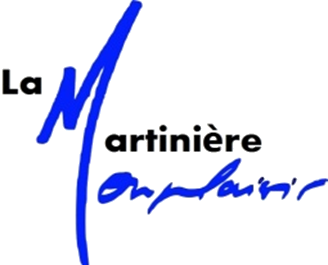
\includegraphics[width=2cm]{png/logo_lycee.png}%
 \end{minipage}}

\fancyhead[C]{\rule{8cm}{.5pt}}

 \fancyhead[R]{%
 \noindent\begin{minipage}[c]{3cm}
 \begin{flushright}
 \footnotesize{\textit{\textsf{\xxtete}}}%
 \end{flushright}
 \end{minipage}
}


\fancyfoot[C]{\rule{12cm}{.5pt}}
\renewcommand{\footrulewidth}{0.2pt}
\fancyfoot[C]{\footnotesize{\bfseries \thepage}}
\fancyfoot[L]{ 
\begin{minipage}[c]{.4\linewidth}
\noindent\footnotesize{{\xxauteur}}
\end{minipage}}


\fancyfoot[R]{\footnotesize{\xxpied}
\ifthenelse{\isodd{\value{page}}}{
\begin{tikzpicture}[overlay]
\node[shape=rectangle, 
      rounded corners = .25 cm,
	  draw= ocre,
	  line width=2pt, 
	  fill = ocre!10,
	  minimum width  = 2.5cm,
	  minimum height = 3cm,] at (\xxposongletx,\xxposonglety) {};
\node at (\xxposonglettext,\xxposonglety) {\rotatebox{90}{\textbf{\large\color{ocre}{\xxonglet}}}};
%{};
\end{tikzpicture}}{}
}
%
%
%
% Removes the header from odd empty pages at the end of chapters
\makeatletter
\renewcommand{\cleardoublepage}{
\clearpage\ifodd\c@page\else
\hbox{}
\vspace*{\fill}
\thispagestyle{empty}
\newpage
\fi}

\fancypagestyle{plain}{%
\fancyhf{} % vide l’en-tête et le pied~de~page.
%\fancyfoot[C]{\bfseries \thepage} % numéro de la page en cours en gras
% et centré en pied~de~page.
\fancyfoot[R]{\footnotesize{\xxpied}}
\fancyfoot[C]{\rule{12cm}{.5pt}}
\renewcommand{\footrulewidth}{0.2pt}
\fancyfoot[C]{\footnotesize{\bfseries \thepage}}
\fancyfoot[L]{ 
\begin{minipage}[c]{.4\linewidth}
\noindent\footnotesize{{\xxauteur}}
\end{minipage}}}



%----------------------------------------------------------------------------------------
%	THEOREM STYLES
%----------------------------------------------------------------------------------------

% Conflit avec la police adobe
%\usepackage{amsmath,amsfonts,amssymb,amsthm} % For math equations, theorems, symbols, etc
\usepackage{amsmath,amsthm}

\newcommand{\intoo}[2]{\mathopen{]}#1\,;#2\mathclose{[}}
\newcommand{\ud}{\mathop{\mathrm{{}d}}\mathopen{}}
\newcommand{\intff}[2]{\mathopen{[}#1\,;#2\mathclose{]}}
%\newtheorem{notation}{Notation}[chapter]
\newtheorem{notation}{Notation}[section]

% Boxed/framed environments
\newtheoremstyle{ocrenumbox}% % Theorem style name
{0pt}% Space above
{0pt}% Space below
{\normalfont}% % Body font
{}% Indent amount
{\small\bf\sffamily\color{ocre}}% % Theorem head font
{\;}% Punctuation after theorem head
{0.25em}% Space after theorem head
{\small\sffamily\color{ocre}\thmname{#1}\nobreakspace\thmnumber%{\@ifnotempty{#1}{}\@upn{#2}}% Theorem text (e.g. Theorem 2.1)
\thmnote{\nobreakspace\the\thm@notefont\sffamily\bfseries\color{black}---\nobreakspace#3.}} % Optional theorem note
\renewcommand{\qedsymbol}{$\blacksquare$}% Optional qed square


% Boite pour les corriges
\newtheoremstyle{correctionbox}% % Theorem style name
{0pt}% Space above
{0pt}% Space below
{\normalfont}% % Body font
{}% Indent amount
{\small\bf\sffamily\color{violet}}% % Theorem head font
{\;}% Punctuation after theorem head
{0.25em}% Space after theorem head
{\small\sffamily\color{ocre}\thmname{#1}\nobreakspace\thmnumber%{\@ifnotempty{#1}{}\@upn{#2}}% Theorem text (e.g. Theorem 2.1)
\thmnote{\nobreakspace\the\thm@notefont\sffamily\bfseries\color{black}---\nobreakspace#3.}} % Optional theorem note
\renewcommand{\qedsymbol}{$\blacksquare$}% Optional qed square



\newtheoremstyle{blacknumex}% Theorem style name
{5pt}% Space above
{5pt}% Space below
{\normalfont}% Body font
{} % Indent amount
{\small\bf\sffamily}% Theorem head font
{\;}% Punctuation after theorem head
{0.25em}% Space after theorem head
{\small\sffamily{\tiny\ensuremath{\blacksquare}}\nobreakspace\thmname{#1}\nobreakspace\thmnumber%{\@ifnotempty{#1}{}\@upn{#2}}% Theorem text (e.g. Theorem 2.1)
\thmnote{\nobreakspace\the\thm@notefont\sffamily\bfseries---\nobreakspace#3.}}% Optional theorem note

\newtheoremstyle{blacknumbox} % Theorem style name
{0pt}% Space above
{0pt}% Space below
{\normalfont}% Body font
{}% Indent amount
{\small\bf\sffamily}% Theorem head font
{\;}% Punctuation after theorem head
{0.25em}% Space after theorem head
{\small\sffamily\thmname{#1}\nobreakspace 
\thmnote{\nobreakspace\the\thm@notefont\sffamily\bfseries---\nobreakspace#3.}}% Optional theorem note

% Non-boxed/non-framed environments
\newtheoremstyle{ocrenum}% % Theorem style name
{5pt}% Space above
{5pt}% Space below
{\normalfont}% % Body font
{}% Indent amount
{\small\bf\sffamily\color{ocre}}% % Theorem head font
{\;}% Punctuation after theorem head
{0.25em}% Space after theorem head
{\small\sffamily\color{ocre}\thmname{#1}\nobreakspace%\thmnumber{\@ifnotempty{#1}{}\@upn{#2}}% Theorem text (e.g. Theorem 2.1)
\thmnote{\nobreakspace\the\thm@notefont\sffamily\bfseries\color{black}---\nobreakspace#3.}} % Optional theorem note
\renewcommand{\qedsymbol}{$\blacksquare$}% Optional qed square
\makeatother

% Environnement pour les titres de parties
\newtheoremstyle{partiebox} 
{0pt}% Space above
{0pt}% Space below
{\normalfont}% Body font
{}% Indent amount
{\small\bf\sffamily}% Theorem head font
{\;}% Punctuation after theorem head
{0.25em}% Space after theorem head




% Defines the theorem text style for each type of theorem to one of the three styles above
\newcounter{dummy} 
\numberwithin{dummy}{section}
\theoremstyle{ocrenumbox}
%\newtheorem{theoremeT}[dummy]{Théorème}
\newtheorem{theoremeT}[dummy]{Théorème}
\newtheorem{resultatT}[dummy]{Résultat}
\newtheorem{savoirT}[dummy]{Savoir}
\newtheorem{methodeT}[dummy]{Méthode}
\newtheorem{objectifT}[dummy]{Objectif}
%\newtheorem{problem}{Problem}[chapter]
\newtheorem{problem}{Problem}[section]
%\newtheorem{exerciseT}{Exercise}[chapter]
\newtheorem{exerciseT}{Exercice}[section]

\theoremstyle{blacknumex}
%\newtheorem{exampleT}{Example}[chapter]
\newtheorem{exempleT}{Exemple}[section]
\newtheorem{termT}{Terminal\\}[section]
\newtheorem{pyT}{Python\\}[section]
\newtheorem{sciT}{Scilab\\}[section]
\newtheorem{pseudoT}{Pseudo Code\\}[section]
\newtheorem{sqlT}{SQL\\}[section]

\theoremstyle{blacknumbox}
%\newtheorem{vocabulary}{Vocabulary}[chapter]
\newtheorem{vocabulary}{Vocabulaire}[section]
%\newtheorem{definitionT}{Definition}[section]
\newtheorem{definitionT}{Définition}[section]
\newtheorem{rappelT}{Rappel}[section]
\newtheorem{demoT}{Démonstration}[section]
\newtheorem{corollaryT}[dummy]{Corollaire}
\newtheorem{hypoT}{Hypothèse(s)}

\theoremstyle{ocrenum}
\newtheorem{proposition}[dummy]{Proposition}

\theoremstyle{partiebox}
\newtheorem{titrepartieT}[]{}
\newtheorem{titrechapitreT}[]{}

\theoremstyle{correctionbox}
\newtheorem{correctionT}[dummy]{\color{violet}{Correction}}

%----------------------------------------------------------------------------------------
%	DEFINITION OF COLORED BOXES
%----------------------------------------------------------------------------------------

\RequirePackage[framemethod=tikz]{mdframed} % Required for creating the theorem, definition, exercise and corollary boxes

% Theorem box
\newmdenv[skipabove=7pt,
skipbelow=7pt,
backgroundcolor=ocre!10,
linecolor=ocre,
innerleftmargin=5pt,
innerrightmargin=5pt,
innertopmargin=5pt,
leftmargin=0cm,
rightmargin=0cm,
innerbottommargin=5pt]{tBox}


% Correction
\newmdenv[skipabove=7pt,
skipbelow=7pt,
backgroundcolor=violet!10,
linecolor=violet,
innerleftmargin=5pt,
innerrightmargin=5pt,
innertopmargin=5pt,
leftmargin=0cm,
rightmargin=0cm,
innerbottommargin=5pt]{coBox}


% Exercise box	  
\newmdenv[skipabove=7pt,
skipbelow=7pt,
rightline=false,
leftline=true,
topline=false,
bottomline=false,
backgroundcolor=ocre!10,
linecolor=ocre,
innerleftmargin=5pt,
innerrightmargin=5pt,
innertopmargin=5pt,
innerbottommargin=5pt,
leftmargin=0cm,
rightmargin=0cm,
linewidth=4pt]{eBox}	

% Definition box
\newmdenv[skipabove=7pt,
skipbelow=7pt,
rightline=false,
leftline=true,
topline=false,
bottomline=false,
backgroundcolor=ocre!10,
linecolor=ocre,
innerleftmargin=5pt,
innerrightmargin=5pt,
innertopmargin=0pt,
leftmargin=0cm,
rightmargin=0cm,
linewidth=4pt,
innerbottommargin=0pt]{dBox}	

% Demonstration box
\newmdenv[skipabove=7pt,
skipbelow=7pt,
rightline=false,
leftline=true,
topline=false,
bottomline=false,
%backgroundcolor=ocre!10,
linecolor=ocre,
innerleftmargin=5pt,
innerrightmargin=5pt,
innertopmargin=0pt,
leftmargin=0cm,
rightmargin=0cm,
linewidth=4pt,
innerbottommargin=0pt]{demoBox}	

% Corollary box
\newmdenv[skipabove=7pt,
skipbelow=7pt,
rightline=false,
leftline=true,
topline=false,
bottomline=false,
linecolor=gray,
backgroundcolor=black!5,
innerleftmargin=5pt,
innerrightmargin=5pt,
innertopmargin=5pt,
leftmargin=0cm,
rightmargin=0cm,
linewidth=4pt,
innerbottommargin=5pt]{cBox}


% Hypothèses
\newmdenv[skipabove=7pt,
skipbelow=7pt,
rightline=false,
leftline=true,
topline=false,
bottomline=false,
linecolor=gray,
backgroundcolor=black!5,
innerleftmargin=5pt,
innerrightmargin=5pt,
innertopmargin=5pt,
leftmargin=0cm,
rightmargin=0cm,
linewidth=4pt,
innerbottommargin=5pt]{hyBox}


% Boite pour le titre de la partie (pBox)
\newmdenv[skipabove=7pt,
skipbelow=7pt,
rightline=true,
leftline=false,
topline=false,
bottomline=false,
linecolor=ocre,
backgroundcolor=none,
innerleftmargin=5pt,
innerrightmargin=5pt,
innertopmargin=5pt,
leftmargin=0cm,
rightmargin=0cm,
linewidth=4pt,
innerbottommargin=5pt]{pBox}

% Boite pour le titre du chapitre (chBox)
\newmdenv[skipabove=7pt,
skipbelow=7pt,
rightline=false,
leftline=true,
topline=false,
bottomline=false,
linecolor=ocre,
%backgroundcolor=black!5,
innerleftmargin=5pt,
innerrightmargin=5pt,
innertopmargin=5pt,
leftmargin=0cm,
rightmargin=0cm,
linewidth=4pt,
innerbottommargin=5pt]{chBox}


% Boite pour les exemples
\newmdenv[skipabove=7pt,
skipbelow=7pt,
rightline=false,
leftline=true,
topline=false,
bottomline=false,
linecolor=gray,
backgroundcolor=white,
innerleftmargin=5pt,
innerrightmargin=5pt,
innertopmargin=5pt,
leftmargin=0cm,
rightmargin=0cm,
linewidth=4pt,
innerbottommargin=5pt]{exBox}

% Boite pour le terminal
\newmdenv[skipabove=7pt,
skipbelow=7pt,
rightline=false,
leftline=true,
topline=false,
bottomline=false,
linecolor=gray,
backgroundcolor=white,
innerleftmargin=5pt,
innerrightmargin=5pt,
innertopmargin=5pt,
leftmargin=0cm,
rightmargin=0cm,
linewidth=4pt,
innerbottommargin=5pt]{termBox}


% Boite pour Python
\newmdenv[skipabove=7pt,
skipbelow=7pt,
rightline=false,
leftline=true,
topline=false,
bottomline=false,
linecolor=gray,
backgroundcolor=white,
innerleftmargin=5pt,
innerrightmargin=5pt,
innertopmargin=0pt,
leftmargin=0cm,
rightmargin=0cm,
linewidth=4pt,
innerbottommargin=5pt]{pyBox}

% Boite pour scilab
\newmdenv[skipabove=7pt,
skipbelow=7pt,
rightline=false,
leftline=true,
topline=false,
bottomline=false,
linecolor=gray,
backgroundcolor=white,
innerleftmargin=5pt,
innerrightmargin=5pt,
innertopmargin=5pt,
leftmargin=0cm,
rightmargin=0cm,
linewidth=4pt,
innerbottommargin=5pt]{sciBox}


% Boite pour pseudo
\newmdenv[skipabove=7pt,
skipbelow=7pt,
rightline=false,
leftline=true,
topline=false,
bottomline=false,
linecolor=gray,
backgroundcolor=white,
innerleftmargin=5pt,
innerrightmargin=5pt,
innertopmargin=5pt,
leftmargin=0cm,
rightmargin=0cm,
linewidth=4pt,
innerbottommargin=5pt]{pseudoBox}

% Boite pour pseudo
\newmdenv[skipabove=7pt,
skipbelow=7pt,
rightline=false,
leftline=true,
topline=false,
bottomline=false,
linecolor=gray,
backgroundcolor=white,
innerleftmargin=5pt,
innerrightmargin=5pt,
innertopmargin=5pt,
leftmargin=0cm,
rightmargin=0cm,
linewidth=4pt,
innerbottommargin=5pt]{sqlBox}


% Creates an environment for each type of theorem and assigns it a theorem text style from the "Theorem Styles" section above and a colored box from above
\newenvironment{theorem}{\begin{tBox}\begin{theoremeT}}{\end{theoremeT}\end{tBox}}
\newenvironment{resultat}{\begin{tBox}\begin{resultatT}}{\end{resultatT}\end{tBox}}
\newenvironment{methode}{\begin{tBox}\begin{methodeT}}{\end{methodeT}\end{tBox}}
\newenvironment{savoir}{\begin{tBox}\begin{savoirT}}{\end{savoirT}\end{tBox}}
\newenvironment{obj}{\begin{tBox}\begin{objectifT}}{\end{objectifT}\end{tBox}}
\newenvironment{corrige}{\begin{coBox}\begin{correctionT}}{\end{correctionT}\end{coBox}}
\newenvironment{exercise}{\begin{eBox}\begin{exerciseT}}{\hfill{\color{ocre}\tiny\ensuremath{\blacksquare}}\end{exerciseT}\end{eBox}}				  
\newenvironment{exercice}{\begin{eBox}\begin{exerciseT}}{\hfill{\color{ocre}\tiny\ensuremath{\blacksquare}}\end{exerciseT}\end{eBox}}				  

\newenvironment{definition}{\begin{dBox}\begin{definitionT}}{\end{definitionT}\end{dBox}}	
\newenvironment{rappel}{\begin{dBox}\begin{rappelT}}{\end{rappelT}\end{dBox}}	
\newenvironment{defi}{\begin{dBox}\begin{definitionT}}{\end{definitionT}\end{dBox}}	
\newenvironment{demo}{\begin{demoBox}\begin{demoT}}{\end{demoT}\end{demoBox}}	
%\newenvironment{exemple}{\begin{exempleT}}{\hfill{\tiny\ensuremath{\blacksquare}}\end{exempleT}}		
\newenvironment{corollary}{\begin{cBox}\begin{corollaryT}}{\end{corollaryT}\end{cBox}}
\newenvironment{hypo}{\begin{hyBox}\begin{hypoT}}{\end{hypoT}\end{hyBox}}	\newenvironment{exemple}{\begin{exBox}\begin{exempleT}}{\hfill{\tiny\ensuremath{\blacksquare}}\end{exempleT}\end{exBox}}	
\newenvironment{titrepartie}{\begin{pBox}\begin{titrepartieT}}{\end{titrepartieT}\end{pBox}}	
\newenvironment{titrechapitre}{\begin{chBox}\begin{titrechapitreT}}{\end{titrechapitreT}\end{chBox}}	

\newenvironment{term}{ \begin{termBox}\begin{termT}}{\end{termT}\end{termBox}}
\newenvironment{py}{ \begin{pyBox}\begin{pyT}}{\end{pyT}\end{pyBox}}
\newenvironment{sci}{ \begin{sciBox}\begin{sciT}}{\end{sciT}\end{sciBox}}
\newenvironment{pseudo}{ \begin{pseudoBox}\begin{pseudoT}}{\end{pseudoT}\end{pseudoBox}}
\newenvironment{envsql}{ \begin{sqlBox}\begin{sqlT}}{\end{sqlT}\end{sqlBox}}


%----------------------------------------------------------------------------------------
%	REMARK ENVIRONMENT
%----------------------------------------------------------------------------------------

\newenvironment{remark}{\par\vspace{10pt}\small % Vertical white space above the remark and smaller font size
\begin{list}{}{
\leftmargin=35pt % Indentation on the left
\rightmargin=25pt}\item\ignorespaces % Indentation on the right
\makebox[-2.5pt]{\begin{tikzpicture}[overlay]
\node[draw=ocre!60,line width=1pt,circle,fill=ocre!25,font=\sffamily\bfseries,inner sep=2pt,outer sep=0pt] at (-15pt,0pt){\textcolor{ocre}{R}};\end{tikzpicture}} % Orange R in a circle
\advance\baselineskip -1pt}{\end{list}\vskip5pt} % Tighter line spacing and white space after remark

\newenvironment{rem}{\par\vspace{10pt}\small % Vertical white space above the remark and smaller font size
\begin{list}{}{
\leftmargin=35pt % Indentation on the left
\rightmargin=25pt}\item\ignorespaces % Indentation on the right
\makebox[-2.5pt]{\begin{tikzpicture}[overlay]
\node[draw=ocre!60,line width=1pt,circle,fill=ocre!25,font=\sffamily\bfseries,inner sep=2pt,outer sep=0pt] at (-15pt,0pt){\textcolor{ocre}{R}};\end{tikzpicture}} % Orange R in a circle
\advance\baselineskip -1pt}{\end{list}\vskip5pt} % Tighter line spacing and white space after remark


\newenvironment{warn}{\par\vspace{10pt}\small % Vertical white space above the remark and smaller font size
\begin{list}{}{
\leftmargin=35pt % Indentation on the left
\rightmargin=25pt}\item\ignorespaces % Indentation on the right
\makebox[-2.5pt]{\begin{tikzpicture}[overlay]
\node[draw=red!60,line width=1pt,circle,fill=red!25,font=\sffamily\bfseries,inner sep=2pt,outer sep=0pt] at (-15pt,0pt){\textcolor{black}{!}};\end{tikzpicture}} % Point d'exclamation dans un cercle
\advance\baselineskip -1pt}{\end{list}\vskip5pt} % Tighter line spacing and white space after remark


%----------------------------------------------------------------------------------------
%	SECTION NUMBERING IN THE MARGIN
%----------------------------------------------------------------------------------------
\setcounter{secnumdepth}{3}
\setcounter{tocdepth}{2}



\makeatletter
\renewcommand{\@seccntformat}[1]{\llap{\textcolor{ocre}{\csname the#1\endcsname}\hspace{1em}}}                    
\renewcommand{\section}{\@startsection{section}{1}{\z@}
{-4ex \@plus -1ex \@minus -.4ex}
{1ex \@plus.2ex }
{\normalfont\large\sffamily\bfseries}}
\renewcommand{\subsection}{\@startsection {subsection}{2}{\z@}
{-3ex \@plus -0.1ex \@minus -.4ex}
{0.5ex \@plus.2ex }
{\normalfont\sffamily\bfseries}}
\renewcommand{\subsubsection}{\@startsection {subsubsection}{3}{\z@}
{-2ex \@plus -0.1ex \@minus -.2ex}
{.2ex \@plus.2ex }
{\normalfont\small\sffamily\bfseries}}                        
\renewcommand\paragraph{\@startsection{paragraph}{4}{\z@}
{-2ex \@plus-.2ex \@minus .2ex}
{.1ex}
{\normalfont\small\sffamily\bfseries}}

%----------------------------------------------------------------------------------------
%	PART HEADINGS
%----------------------------------------------------------------------------------------


%----------------------------------------------------------------------------------------
%	CHAPTER HEADINGS
%----------------------------------------------------------------------------------------

% \newcommand{\thechapterimage}{}%
% \newcommand{\chapterimage}[1]{\renewcommand{\thechapterimage}{#1}}%
% \def\@makechapterhead#1{%
% {\parindent \z@ \raggedright \normalfont
% \ifnum \c@secnumdepth >\m@ne
% \if@mainmatter
% \begin{tikzpicture}[remember picture,overlay]
% \node at (current page.north west)
% {\begin{tikzpicture}[remember picture,overlay]
% \node[anchor=north west,inner sep=0pt] at (0,0) {\includegraphics[width=\paperwidth]{\thechapterimage}};
% \draw[anchor=west] (\Gm@lmargin,-9cm) node [line width=2pt,rounded corners=15pt,draw=ocre,fill=white,fill opacity=0.5,inner sep=15pt]{\strut\makebox[22cm]{}};
% \draw[anchor=west] (\Gm@lmargin+.3cm,-9cm) node {\huge\sffamily\bfseries\color{black}\thechapter. #1\strut};
% \end{tikzpicture}};
% \end{tikzpicture}
% \else
% \begin{tikzpicture}[remember picture,overlay]
% \node at (current page.north west)
% {\begin{tikzpicture}[remember picture,overlay]
% \node[anchor=north west,inner sep=0pt] at (0,0) {\includegraphics[width=\paperwidth]{\thechapterimage}};
% \draw[anchor=west] (\Gm@lmargin,-9cm) node [line width=2pt,rounded corners=15pt,draw=ocre,fill=white,fill opacity=0.5,inner sep=15pt]{\strut\makebox[22cm]{}};
% \draw[anchor=west] (\Gm@lmargin+.3cm,-9cm) node {\huge\sffamily\bfseries\color{black}#1\strut};
% \end{tikzpicture}};
% \end{tikzpicture}
% \fi\fi\par\vspace*{270\p@}}}

%-------------------------------------------

\def\@makeschapterhead#1{%
\begin{tikzpicture}[remember picture,overlay]
\node at (current page.north west)
{\begin{tikzpicture}[remember picture,overlay]
\node[anchor=north west,inner sep=0pt] at (0,0) {\includegraphics[width=\paperwidth]{\thechapterimage}};
\draw[anchor=west] (\Gm@lmargin,-9cm) node [line width=2pt,rounded corners=15pt,draw=ocre,fill=white,fill opacity=0.5,inner sep=15pt]{\strut\makebox[22cm]{}};
\draw[anchor=west] (\Gm@lmargin+.3cm,-9cm) node {\huge\sffamily\bfseries\color{black}#1\strut};
\end{tikzpicture}};
\end{tikzpicture}
\par\vspace*{270\p@}}
\makeatother

%----------------------------------------------------------------------------------------
%	HYPERLINKS IN THE DOCUMENTS
%----------------------------------------------------------------------------------------


%\hypersetup{hidelinks,backref=true,pagebackref=true,hyperindex=true,colorlinks=false,breaklinks=true,urlcolor= ocre,bookmarks=true,bookmarksopen=false,pdftitle={Title},pdfauthor={Author}}
%\usepackage{bookmark}
%\bookmarksetup{
%open,
%numbered,
%addtohook={%
%\ifnum\bookmarkget{level}=0 % chapter
%\bookmarksetup{bold}%
%\fi
%\ifnum\bookmarkget{level}=-1 % part
%\bookmarksetup{color=ocre,bold}%
%\fi
%}
%}

%----------------------------------------------------------------------------------------
%	
%----------------------------------------------------------------------------------------

\newcommand{\thechapterimage}{}%
\newcommand{\chapterimage}[1]{\renewcommand{\thechapterimage}{#1}}%
\def\@makechapterhead#1{%
{\parindent \z@ \raggedright \normalfont
\begin{tikzpicture}[remember picture,overlay]
\node at (current page.north west)
{\begin{tikzpicture}[remember picture,overlay]
\node[anchor=north west,inner sep=0pt] at (0,0) {\includegraphics[width=\paperwidth]{\thechapterimage}};
%\draw[anchor=west] (\Gm@lmargin,-9cm) node [line width=2pt,rounded corners=15pt,draw=ocre,fill=white,fill opacity=0.5,inner sep=15pt]{\strut\makebox[22cm]{}};
%\draw[anchor=west] (\Gm@lmargin+.3cm,-9cm) node {\huge\sffamily\bfseries\color{black}\thechapter. #1\strut};
\end{tikzpicture}};
\end{tikzpicture}
\par\vspace*{270\p@}
}}

 \newcounter{exo}


\makeatletter             
\renewcommand{\subparagraph}{\@startsection{exo}{5}{\z@}%
                                    {-2ex \@plus-.2ex \@minus .2ex}%
                                    {0ex}%               
{\normalfont\bfseries Question \hspace{.7cm} }}
%M\makeatother
\renewcommand{\thesubparagraph}{\arabic{subparagraph}} 
\makeatletter


%%%%% Environnement pour inclure du code
%%\usepackage{textcomp}
%%\usepackage[french]{algorithm2e}
%%\usepackage{listings}
%%\lstloadlanguages{R}   % pour regler les pb d accent utf8 dans les codes
%%\lstset{language=R} % pour regler les pb d accent utf8 dans les codes
%\renewcommand{\lstlistlistingname}{Listings}
%\renewcommand{\lstlistingname}{Listing}
%
%\SetKwBlock{Fonction}{Début Fonction}{Fin Fonction}
%\SetKwComment{Comment}{start}{end}
%
%\definecolor{Bleu}{rgb}{0.1,0.1,1.0}
%\definecolor{Noir}{rgb}{0,0,0}
%\definecolor{Grau}{rgb}{0.5,0.5,0.5}
%\definecolor{DunkelGrau}{rgb}{0.15,0.15,0.15}
%\definecolor{Hellbraun}{rgb}{0.5,0.25,0.0}
%\definecolor{Magenta}{rgb}{1.0,0.0,1.0}
%\definecolor{Gris}{gray}{0.5}
%\definecolor{Vert}{rgb}{0,0.5,0}
%\definecolor{SourceHintergrund}{rgb}{1,1.0,0.95}
%
%
%\lstnewenvironment{python}[1][]{
%\lstset{
%%escapeinside={\%*}{*)},
%inputencoding=utf8,   % pour regler les pb d accent utf8 dans les codes
%extendedchars=true,   % pour regler les pb d accent utf8 dans les codes
%language=python,
%basicstyle=\ttfamily\footnotesize, 	
%stringstyle=\color{red}, 
%showstringspaces=false, 
%alsoletter={1234567890},
%otherkeywords={\ , \}, \{},
%keywordstyle=\color{blue},
%emph={access,and,break,class,continue,def,del,elif ,else,
%except,exec,finally,for,from,global,if,import,in,i s,
%lambda,not,or,pass,print,raise,return,try,while},
%emphstyle=\color{black}\bfseries,
%emph={[2]True, False, None, self},
%emphstyle=[2]\color{black},
%emph={[3]from, import, as},
%emphstyle=[3]\color{blue},
%upquote=true,
%columns=flexible, % pour empecher d'avoir un espacement mono
%morecomment=[s]{"""}{"""},
%commentstyle=\color{Hellbraun}\slshape, 
%%emph={[4]1, 2, 3, 4, 5, 6, 7, 8, 9, 0},
%emphstyle=[4]\color{blue},
%literate=*{:}{{\textcolor{blue}:}}{1}
%{=}{{\textcolor{blue}=}}{1}
%{-}{{\textcolor{blue}-}}{1}
%{+}{{\textcolor{blue}+}}{1}
%{*}{{\textcolor{blue}*}}{1}
%{!}{{\textcolor{blue}!}}{1}
%{(}{{\textcolor{blue}(}}{1}
%{)}{{\textcolor{blue})}}{1}
%{[}{{\textcolor{blue}[}}{1}
%{]}{{\textcolor{blue}]}}{1}
%{<}{{\textcolor{blue}<}}{1}
%{>}{{\textcolor{blue}>}}{1}
%{COMPLETER}{{\textcolor{red}COMPLETER}}{1},
%literate=%
%            {é}{{\'{e}}}1
%            {è}{{\`{e}}}1
%            {ê}{{\^{e}}}1
%            {ë}{{\¨{e}}}1
%            {û}{{\^{u}}}1
%            {ù}{{\`{u}}}1
%            {â}{{\^{a}}}1
%            {à}{{\`{a}}}1
%            {î}{{\^{i}}}1
%            {ç}{{\c{c}}}1
%            {Ç}{{\c{C}}}1
%            {É}{{\'{E}}}1
%            {Ê}{{\^{E}}}1
%            {À}{{\`{A}}}1
%            {Â}{{\^{A}}}1
%            {Î}{{\^{I}}}1, % pour regler les pb d accent utf8 dans les codes
%%framexleftmargin=1mm, framextopmargin=1mm, frame=shadowbox, rulesepcolor=\color{blue},#1
%%backgroundcolor=\color{SourceHintergrund}, 
%%framexleftmargin=1mm, framexrightmargin=1mm, framextopmargin=1mm, frame=single, framerule=1pt, rulecolor=\color{black},#1
%}}{}
%
%
%
%\lstnewenvironment{scilab}[1][]{
%\lstset{
%language=scilab,
%basicstyle=\sffamily\footnotesize, 	
%stringstyle=\color{red}, 
%showstringspaces=false, 
%alsoletter={1234567890},
%otherkeywords={\ , \}, \{},
%keywordstyle=\color{blue},
%emph={access,and,break,class,continue,def,del,elif ,else,
%except,exec,finally,for,from,global,if,import,in,i s,
%lambda,not,or,pass,print,raise,return,try,while,Debut},
%emphstyle=\color{black}\bfseries,
%emph={[2]True, False, None, self},
%emphstyle=[2]\color{black},
%emph={[3]from, import, as},
%emphstyle=[3]\color{blue},
%upquote=true,
%columns=flexible, % pour empecher d'avoir un espacement mono
%morecomment=[s]{"""}{"""},
%commentstyle=\color{Hellbraun}\slshape, 
%%emph={[4]1, 2, 3, 4, 5, 6, 7, 8, 9, 0},
%emphstyle=[4]\color{blue},
%literate=*{:}{{\textcolor{blue}:}}{1}
%{=}{{\textcolor{blue}=}}{1}
%{-}{{\textcolor{blue}-}}{1}
%{+}{{\textcolor{blue}+}}{1}
%{*}{{\textcolor{blue}*}}{1}
%{!}{{\textcolor{blue}!}}{1}
%{(}{{\textcolor{blue}(}}{1}
%{)}{{\textcolor{blue})}}{1}
%{[}{{\textcolor{blue}[}}{1}
%{]}{{\textcolor{blue}]}}{1}
%{<}{{\textcolor{blue}<}}{1}
%{>}{{\textcolor{blue}>}}{1},
%%framexleftmargin=1mm, framextopmargin=1mm, frame=shadowbox, rulesepcolor=\color{blue},#1
%%backgroundcolor=\color{SourceHintergrund}, 
%%framexleftmargin=1mm, framexrightmargin=1mm, framextopmargin=1mm, frame=single, framerule=1pt, rulecolor=\color{black},#1
%}}{}
%
%
%\lstdefinestyle{stylepython}{%
%escapeinside={\%*}{*)},
%inputencoding=utf8,   % pour regler les pb d accent utf8 dans les codes
%extendedchars=true,   % pour regler les pb d accent utf8 dans les codes
%language=python,
%basicstyle=\sffamily\footnotesize, 	
%stringstyle=\color{red}, 
%showstringspaces=false, 
%alsoletter={1234567890},
%otherkeywords={\ , \}, \{},
%keywordstyle=\color{blue},
%emph={access,and,break,class,continue,def,del,elif ,else,
%except,exec,finally,for,from,global,if,import,in,i s,
%lambda,not,or,pass,print,raise,return,try,while},
%emphstyle=\color{black}\bfseries,
%emph={[2]True, False, None, self},
%emphstyle=[2]\color{green},
%emph={[3]from, import, as},
%emphstyle=[3]\color{blue},
%upquote=true,
%columns=flexible, % pour empecher d'avoir un espacement mono
%morecomment=[s]{"""}{"""},
%commentstyle=\color{Hellbraun}\slshape, 
%%emph={[4]1, 2, 3, 4, 5, 6, 7, 8, 9, 0},
%emphstyle=[4]\color{blue},
%literate=*{:}{{\textcolor{blue}:}}{1}
%{=}{{\textcolor{blue}=}}{1}
%{-}{{\textcolor{blue}-}}{1}
%{+}{{\textcolor{blue}+}}{1}
%{*}{{\textcolor{blue}*}}{1}
%{!}{{\textcolor{blue}!}}{1}
%{(}{{\textcolor{blue}(}}{1}
%{)}{{\textcolor{blue})}}{1}
%{[}{{\textcolor{blue}[}}{1}
%{]}{{\textcolor{blue}]}}{1}
%{<}{{\textcolor{blue}<}}{1}
%{>}{{\textcolor{blue}>}}{1}
%{COMPLETER}{{\textcolor{red}COMPLETER}}{1},
%literate=%
%            {é}{{\'{e}}}1
%            {è}{{\`{e}}}1
%            {ê}{{\^{e}}}1
%            {ë}{{\¨{e}}}1
%            {û}{{\^{u}}}1
%            {ù}{{\`{u}}}1
%            {â}{{\^{a}}}1
%            {à}{{\`{a}}}1
%            {î}{{\^{i}}}1
%            {ç}{{\c{c}}}1
%            {Ç}{{\c{C}}}1
%            {É}{{\'{E}}}1
%            {Ê}{{\^{E}}}1
%            {À}{{\`{A}}}1
%            {Â}{{\^{A}}}1
%            {Î}{{\^{I}}}1,
%%numbers=left,                    % where to put the line-numbers; possible values are (none, left, right)
%%numbersep=5pt,                   % how far the line-numbers are from the code
%%numberstyle=\tiny\color{mygray}, % the style that is used for the line-numbers
%}
%
%
%
%\lstnewenvironment{termi}[1][]{
%\lstset{
%language=scilab,
%basicstyle=\sffamily\footnotesize, 	
%stringstyle=\color{red}, 
%showstringspaces=false, 
%alsoletter={1234567890},
%otherkeywords={\ , \}, \{},
%keywordstyle=\color{blue},
%emph={access,and,break,class,continue,def,del,elif ,else,
%except,exec,finally,for,from,global,if,import,in,i s,
%lambda,not,or,pass,print,raise,return,try,while,Debut},
%emphstyle=\color{black}\bfseries,
%emph={[2]True, False, None, self},
%emphstyle=[2]\color{green},
%emph={[3]from, import, as},
%emphstyle=[3]\color{blue},
%upquote=true,
%columns=flexible, % pour empecher d'avoir un espacement mono
%morecomment=[s]{"""}{"""},
%commentstyle=\color{Hellbraun}\slshape, 
%%emph={[4]1, 2, 3, 4, 5, 6, 7, 8, 9, 0},
%emphstyle=[4]\color{blue},
%literate=*{:}{{\textcolor{blue}:}}{1}
%{=}{{\textcolor{blue}=}}{1}
%{-}{{\textcolor{blue}-}}{1}
%{+}{{\textcolor{blue}+}}{1}
%{*}{{\textcolor{blue}*}}{1}
%{!}{{\textcolor{blue}!}}{1}
%{(}{{\textcolor{blue}(}}{1}
%{)}{{\textcolor{blue})}}{1}
%{[}{{\textcolor{blue}[}}{1}
%{]}{{\textcolor{blue}]}}{1}
%{<}{{\textcolor{blue}<}}{1}
%{>}{{\textcolor{blue}>}}{1},
%%framexleftmargin=1mm, framextopmargin=1mm, frame=shadowbox, rulesepcolor=\color{blue},#1
%%backgroundcolor=\color{SourceHintergrund}, 
%%framexleftmargin=1mm, framexrightmargin=1mm, framextopmargin=1mm, frame=single, framerule=1pt, rulecolor=\color{black},#1
%}}{}
%
%
%\lstnewenvironment{sql}[1][]{
%\lstset{
%%escapeinside={\%*}{*)},
%%inputencoding=utf8,   % pour regler les pb d accent utf8 dans les codes
%%extendedchars=true,   % pour regler les pb d accent utf8 dans les codes
%language=sql,
%basicstyle=\sffamily\footnotesize, 	
%stringstyle=\color{red}, 
%showstringspaces=false, 
%alsoletter={1234567890},
%otherkeywords={\ , \}, \{},
%keywordstyle=\color{blue},
%emph={access,and,break,class,continue,def,del,elif ,else,
%except,exec,finally,for,from,global,if,import,in,i s,
%lambda,not,or,pass,print,raise,return,try,while},
%emphstyle=\color{black}\bfseries,
%emph={[2]True, False, None, self},
%emphstyle=[2]\color{black},
%emph={[3]from, import, as},
%emphstyle=[3]\color{blue},
%upquote=true,
%columns=flexible, % pour empecher d'avoir un espacement mono
%morecomment=[s]{"""}{"""},
%commentstyle=\color{Hellbraun}\slshape, 
%%emph={[4]1, 2, 3, 4, 5, 6, 7, 8, 9, 0},
%emphstyle=[4]\color{blue},
%literate=*{:}{{\textcolor{blue}:}}{1}
%{=}{{\textcolor{blue}=}}{1}
%{-}{{\textcolor{blue}-}}{1}
%{+}{{\textcolor{blue}+}}{1}
%{*}{{\textcolor{blue}*}}{1}
%{!}{{\textcolor{blue}!}}{1}
%{(}{{\textcolor{blue}(}}{1}
%{)}{{\textcolor{blue})}}{1}
%{[}{{\textcolor{blue}[}}{1}
%{]}{{\textcolor{blue}]}}{1}
%{<}{{\textcolor{blue}<}}{1}
%{>}{{\textcolor{blue}>}}{1}
%{COMPLETER}{{\textcolor{red}COMPLETER}}{1},
%literate=%
%            {é}{{\'{e}}}1
%            {è}{{\`{e}}}1
%            {ê}{{\^{e}}}1
%            {ë}{{\¨{e}}}1
%            {û}{{\^{u}}}1
%            {ù}{{\`{u}}}1
%            {â}{{\^{a}}}1
%            {à}{{\`{a}}}1
%            {î}{{\^{i}}}1
%            {ç}{{\c{c}}}1
%            {Ç}{{\c{C}}}1
%            {É}{{\'{E}}}1
%            {Ê}{{\^{E}}}1
%            {À}{{\`{A}}}1
%            {Â}{{\^{A}}}1
%            {Î}{{\^{I}}}1, % pour regler les pb d accent utf8 dans les codes
%%framexleftmargin=1mm, framextopmargin=1mm, frame=shadowbox, rulesepcolor=\color{blue},#1
%%backgroundcolor=\color{SourceHintergrund}, 
%%framexleftmargin=1mm, framexrightmargin=1mm, framextopmargin=1mm, frame=single, framerule=1pt, rulecolor=\color{black},#1
%}}{}


% Définition des booleéns
\newif\iffiche
\newif\ifprof
\newif\iftd
\newif\ifcours

%%%%%%%%%%%%
% Définition des vecteurs 
%%%%%%%%%%%%
\newcommand{\vect}[1]{\overrightarrow{#1}}
\newcommand{\axe}[2]{\left(#1,\vect{#2}\right)}
\newcommand{\couple}[2]{\left(#1,\vect{#2}\right)}
\newcommand{\angl}[2]{\left(\vect{#1},\vect{#2}\right)}

\newcommand{\rep}[1]{\mathcal{R}_{#1}}
\newcommand{\quadruplet}[4]{\left(#1;#2,#3,#4 \right)}
\newcommand{\repere}[4]{\left(#1;\vect{#2},\vect{#3},\vect{#4} \right)}
\newcommand{\base}[3]{\left(\vect{#1},\vect{#2},\vect{#3} \right)}


\newcommand{\vx}[1]{\vect{x_{#1}}}
\newcommand{\vy}[1]{\vect{y_{#1}}}
\newcommand{\vz}[1]{\vect{z_{#1}}}

\newcommand{\norm}[1]{\ensuremath{\left\Vert {#1}\right\Vert}}
\newcommand{\Ker}{\mathop{\mathrm{Ker}}\nolimits}

% d droit pour le calcul différentiel
\newcommand{\dd}{\text{d}}

\newcommand{\inertie}[2]{I_{#1}\left( #2\right)}
\newcommand{\matinertie}[7]{
\begin{pmatrix}
#1 & #6 & #5 \\
#6 & #2 & #4 \\
#5 & #4 & #3 \\
\end{pmatrix}_{#7}}
%%%%%%%%%%%%
% Définition des torseurs 
%%%%%%%%%%%%

\newcommand{\ec}[2]{%
\mathcal{E}_c\left(#1/#2\right)}

\newcommand{\pext}[3]{%
\mathcal{P}\left(#1\rightarrow#2/#3\right)}

\newcommand{\pint}[3]{%
\mathcal{P}\left(#1 \stackrel{\text{#3}}{\leftrightarrow} #2\right)}


 \newcommand{\torseur}[1]{%
\left\{{#1}\right\}
}

\newcommand{\torseurcin}[3]{%
\left\{\mathcal{#1} \left(#2/#3 \right) \right\}
}

\newcommand{\torseurci}[2]{%
\left\{\sigma \left(#1/#2 \right) \right\}
}
\newcommand{\torseurdyn}[2]{%
\left\{\mathcal{D} \left(#1/#2 \right) \right\}
}


\newcommand{\torseurstat}[3]{%
\left\{\mathcal{#1} \left(#2\rightarrow #3 \right) \right\}
}


 \newcommand{\torseurc}[8]{%
%\left\{#1 \right\}=
\left\{
{#1}
\right\}
 = 
\left\{%
\begin{array}{cc}%
{#2} & {#5}\\%
{#3} & {#6}\\%
{#4} & {#7}\\%
\end{array}%
\right\}_{#8}%
}

 \newcommand{\torseurcol}[7]{
\left\{%
\begin{array}{cc}%
{#1} & {#4}\\%
{#2} & {#5}\\%
{#3} & {#6}\\%
\end{array}%
\right\}_{#7}%
}

 \newcommand{\torseurl}[3]{%
%\left\{\mathcal{#1}\right\}_{#2}=%
\left\{%
\begin{array}{l}%
{#1} \\%
{#2} %
\end{array}%
\right\}_{#3}%
}

% Vecteur vitesse
 \newcommand{\vectv}[3]{%
\vect{V\left( {#1} \in {#2}/{#3}\right)}
}

% Vecteur force
\newcommand{\vectf}[2]{%
\vect{R\left( {#1} \rightarrow {#2}\right)}
}

% Vecteur moment stat
\newcommand{\vectm}[3]{%
\vect{\mathcal{M}\left( {#1}, {#2} \rightarrow {#3}\right)}
}




% Vecteur résultante cin
\newcommand{\vectrc}[2]{%
\vect{R_c \left( {#1}/ {#2}\right)}
}
% Vecteur moment cin
\newcommand{\vectmc}[3]{%
\vect{\sigma \left( {#1}, {#2} /{#3}\right)}
}


% Vecteur résultante dyn
\newcommand{\vectrd}[2]{%
\vect{R_d \left( {#1}/ {#2}\right)}
}
% Vecteur moment dyn
\newcommand{\vectmd}[3]{%
\vect{\delta \left( {#1}, {#2} /{#3}\right)}
}

% Vecteur accélération
 \newcommand{\vectg}[3]{%
\vect{\Gamma \left( {#1} \in {#2}/{#3}\right)}
}

% Vecteur omega
 \newcommand{\vecto}[2]{%
\vect{\Omega\left( {#1}/{#2}\right)}
}
% }$$\left\{\mathcal{#1} \right\}_{#2} =%
% \left\{%
% \begin{array}{c}%
%  #3 \\%
%  #4 %
% \end{array}%
% \right\}_{#5}}

\newcommand{\N}{\mathbb{N}}
\newcommand{\Z}{\mathbb{Z}}
\newcommand{\R}{\mathbb{R}}
\newcommand{\C}{\mathbb{C}}
\newcommand{\K}{\mathbb{K}}

\newcommand{\cA}{\mathscr{A}}
\newcommand{\cM}{\mathscr{M}}
\newcommand{\cL}{\mathscr{L}}
\newcommand{\cS}{\mathscr{S}}

\newcommand{\python}{\texttt{Python}}

\newcommand{\z}[1]{\Z_{#1}}
\newcommand{\ztimes}[1]{\Z_{#1}^{\times}}
\newcommand{\ii}[1]{[\![#1[\![}
\newcommand{\iif}[1]{[\![#1]\!]}
\newcommand{\llbr}{\ensuremath{\llbracket}}
\newcommand{\rrbr}{\ensuremath{\rrbracket}}
%\newcommand{\p}[1]{\left(#1\right)}
\newcommand{\ens}[1]{\left\{ #1 \right\}}
\newcommand{\croch}[1]{\left[ #1 \right]}
%\newcommand{\of}[1]{\lstinline{#1}}
% \newcommand{\py}[2]{%
%   \begin{tabular}{|l}
%     \lstinline+>>>+\textbf{\of{#1}}\\
%     \of{#2}
%   \end{tabular}\par{}
% }
\newcommand{\floor}[1]{\left\lfloor#1\right\rfloor}
\newcommand{\ceil}[1]{\left\lceil#1\right\rceil}
\newcommand{\abs}[1]{\left|#1\right|}


% Binaire, octal, hexa
\newcommand{\hex}[1]{\underline{\text{\texttt{#1}}}_{16}}
\newcommand{\oct}[1]{\underline{\text{\texttt{#1}}}_{8}}
\newcommand{\bin}[1]{\underline{\text{\texttt{#1}}}_{2}}
\DeclareMathOperator{\mmod}{\texttt{\%}}


% Fonctions et systèmes
\newcommand{\fct}[5][t]{%
  \begin{array}[#1]{rcl}
    #2 & \rightarrow & #3\\
    #4 & \mapsto     & #5\\
  \end{array}
}
\newcommand{\fonction}[5]{#1 : \left\{\begin{array}{rcl} #2& \longrightarrow &#3 \\ #4 &\longmapsto & #5\end{array}\right.}
\newenvironment{systeme}{\left\{ \begin{array}{rcl}}{\end{array}\right.}

% Matrices
\newcommand{\mat}[1]{
  \begin{pmatrix}
    #1
  \end{pmatrix}
}
\newcommand{\inv}{\ensuremath{^{-1}}}
\newcommand{\bpm}{\begin{pmatrix}}
\newcommand{\epm}{\end{pmatrix}}
\usepackage{multicol}
\usepackage{standalone}
\standaloneconfig{mode=buildnew}
\usepackage{siunitx}
\usepackage{wrapfig}
\fichetrue

%\fichefalse

%\proftrue
%\proffalse

\tdtrue
%\tdfalse

\courstrue
\coursfalse

\def\discipline{Sciences \\Industrielles de \\ l'Ingénieur}
\def\xxtete{Sciences Industrielles de l'Ingénieur}

\def\classe{PSI$\star$}
\def\xxnumpartie{Cy 1 \& 2}
\def\xxpartie{Modéliser le comportement linéaire et non linéaire des systèmes multiphysiques\\
Modéliser les systèmes asservis dans le but de prévoir leur comportement}


\def\xxnumchapitre{}%}Chapitre 1 \vspace{.2cm}}
\def\xxchapitre{}%\hspace{.12cm} Modélisation multiphysique}


\def\xxtitreexo{\noindent }%Micromanipulateur compact pour la chirurgie endoscopique \\ Direction Automobile Découplée}%Motorisation du moteur Haibike}
\def\xxsourceexo{}%\hspace{.2cm} \footnotesize{Mines Ponts 2016 -- Banque PT SI A 2017 }}


\def\xxposongletx{2}
\def\xxposonglettext{1.45}
\def\xxposonglety{20}
%\def\xxonglet{Part. 1 -- Ch. 3}
\def\xxonglet{Cy 1 \& 2}

\def\xxactivite{DS 2}
\def\xxauteur{\textsl{Xavier Pessoles}}

\def\xxcompetences{%
\textsl{%
\textbf{Savoirs et compétences :}\\
%Les sources sont associées par un \emph{hacheur série}. La détermination des grandeurs électriques associées à ce montage permet de conclure vis à vis du cahier des charges.
%\noindent \textbf{Résoudre :} à partir des modèles retenus :
%\begin{itemize}[label=\ding{112},font=\color{ocre}] 
%\item choisir une méthode de résolution analytique, graphique, numérique;
%\item mettre en \oe{}uvre une méthode de résolution.
%\end{itemize}
%\begin{itemize}[label=\ding{112},font=\color{ocre}] 
%\item \textit{Rés -- C1.1 :} Loi entrée sortie géométrique et cinématique -- Fermeture géométrique.
%\end{itemize}
%
%\noindent \textit{Mod2 -- C4.1 :} Représentation par schéma-blocs.
}}

\def\xxfigures{
%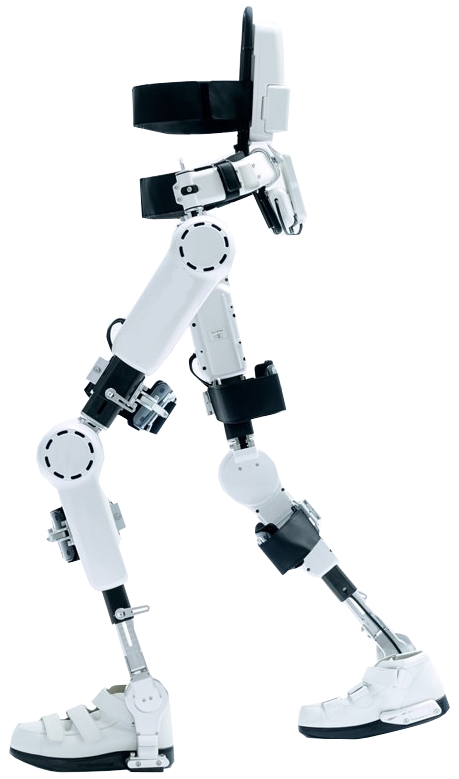
\includegraphics[width=.9\linewidth]{images/fig_01}
}%figues de la page de garde


\def\xxpied{%
Cycle 1 \& 2\\
\xxactivite%
}

\setcounter{secnumdepth}{5}
%---------------------------------------------------------------------------

\usepackage{pgfplots}
\begin{document}
%\defimages{images}
%\chapterimage{png/Fond_Cin}
\pagestyle{empty}


%%%%%%%% PAGE DE GARDE COURS
\ifcours
\begin{tikzpicture}[remember picture,overlay]
\node at (current page.north west)
{\begin{tikzpicture}[remember picture,overlay]
\node[anchor=north west,inner sep=0pt] at (0,0) {\includegraphics[width=\paperwidth]{\thechapterimage}};
\draw[anchor=west] (-2cm,-8cm) node [line width=2pt,rounded corners=15pt,draw=ocre,fill=white,fill opacity=0.6,inner sep=40pt]{\strut\makebox[22cm]{}};
\draw[anchor=west] (1cm,-8cm) node {\huge\sffamily\bfseries\color{black} %
\begin{minipage}{1cm}
\rotatebox{90}{\LARGE\sffamily\textsc{\color{ocre}\textbf{\xxnumpartie}}}
\end{minipage} \hfill
\begin{minipage}[c]{14cm}
\begin{titrepartie}
\begin{flushright}
\renewcommand{\baselinestretch}{1.1} 
\Large\sffamily\textsc{\textbf{\xxpartie}}
\renewcommand{\baselinestretch}{1} 
\end{flushright}
\end{titrepartie}
\end{minipage} \hfill
\begin{minipage}[c]{3.5cm}
{\large\sffamily\textsc{\textbf{\color{ocre} \discipline}}}
\end{minipage} 
 };
\end{tikzpicture}};
\end{tikzpicture}


\begin{tikzpicture}[overlay]
\node[shape=rectangle, 
      rounded corners = .25 cm,
	  draw= ocre,
	  line width=2pt, 
	  fill = ocre!10,
	  minimum width  = 2.5cm,
	  minimum height = 3cm,] at (18cm,0) {};
\node at (17.7cm,0) {\rotatebox{90}{\textbf{\Large\color{ocre}{\classe}}}};
%{};
\end{tikzpicture}

\vspace{3.5cm}

\begin{tikzpicture}[remember picture,overlay]
\draw[anchor=west] (-2cm,-6cm) node {\huge\sffamily\bfseries\color{black} %
\begin{minipage}{2cm}
\begin{center}
\LARGE\sffamily\textsc{\color{ocre}\textbf{\xxactivite}}
\end{center}
\end{minipage} \hfill
\begin{minipage}[c]{15cm}
\begin{titrechapitre}
\renewcommand{\baselinestretch}{1.1} 
\Large\sffamily\textsc{\textbf{\xxnumchapitre}}

\Large\sffamily\textsc{\textbf{\xxchapitre}}
\vspace{.5cm}

\renewcommand{\baselinestretch}{1} 
\normalsize\normalfont
\xxcompetences
\end{titrechapitre}
\end{minipage}  };
\end{tikzpicture}
\vfill

\begin{flushright}
\begin{minipage}[c]{.3\linewidth}
\begin{center}
\xxfigures
\end{center}
\end{minipage}\hfill
\begin{minipage}[c]{.6\linewidth}
\startcontents
\printcontents{}{1}{}
\end{minipage}
\end{flushright}

\begin{tikzpicture}[remember picture,overlay]
\draw[anchor=west] (4.5cm,-.7cm) node {
\begin{minipage}[c]{.2\linewidth}
\begin{flushright}

\includegraphics[width=2cm]{png/logoCC}
\end{flushright}
\end{minipage}
\begin{minipage}[c]{.2\linewidth}
\textsl{\xxauteur} \\
\textsl{\classe}
\end{minipage}
 };
\end{tikzpicture}
\newpage
\pagestyle{fancy}

\newpage
\pagestyle{fancy}

\else
\fi


%%%%%%%% PAGE DE GARDE TD
\iftd
%\begin{tikzpicture}[remember picture,overlay]
%\node at (current page.north west)
%{\begin{tikzpicture}[remember picture,overlay]
%\draw[anchor=west] (-2cm,-3.25cm) node [line width=2pt,rounded corners=15pt,draw=ocre,fill=white,fill opacity=0.6,inner sep=40pt]{\strut\makebox[22cm]{}};
%\draw[anchor=west] (1cm,-3.25cm) node {\huge\sffamily\bfseries\color{black} %
%\begin{minipage}{1cm}
%\rotatebox{90}{\LARGE\sffamily\textsc{\color{ocre}\textbf{\xxnumpartie}}}
%\end{minipage} \hfill
%\begin{minipage}[c]{13.5cm}
%\begin{titrepartie}
%\begin{flushright}
%\renewcommand{\baselinestretch}{1.1} 
%\Large\sffamily\textsc{\textbf{\xxpartie}}
%\renewcommand{\baselinestretch}{1} 
%\end{flushright}
%\end{titrepartie}
%\end{minipage} \hfill
%\begin{minipage}[c]{3.5cm}
%{\large\sffamily\textsc{\textbf{\color{ocre} \discipline}}}
%\end{minipage} 
% };
%\end{tikzpicture}};
%\end{tikzpicture}

%%%%%%%%%% PAGE DE GARDE TD %%%%%%%%%%%%%%%
%\begin{tikzpicture}[overlay]
%\node[shape=rectangle, 
%      rounded corners = .25 cm,
%	  draw= ocre,
%	  line width=2pt, 
%	  fill = ocre!10,
%	  minimum width  = 2.5cm,
%	  minimum height = 2.5cm,] at (18.5cm,0) {};
%\node at (17.7cm,0) {\rotatebox{90}{\textbf{\Large\color{ocre}{\classe}}}};
%%{};
%\end{tikzpicture}

% PARTIE ET CHAPITRE
%\begin{tikzpicture}[remember picture,overlay]
%\draw[anchor=west] (-1cm,-2.1cm) node {\large\sffamily\bfseries\color{black} %
%\begin{minipage}[c]{15cm}
%\begin{flushleft}
%\xxnumchapitre \\
%\xxchapitre
%\end{flushleft}
%\end{minipage}  };
%\end{tikzpicture}

% Bandeau titre exo
\begin{tikzpicture}[remember picture,overlay]
\draw[anchor=west] (-2cm,-6cm) node {\huge\sffamily\bfseries\color{black} %
\begin{minipage}{5cm}
\begin{center}
\LARGE\sffamily\color{ocre}\textbf{\textsc{\xxactivite}}

\begin{center}
\xxfigures
\end{center}

\end{center}
\end{minipage} \hfill
\begin{minipage}[c]{12cm}
\begin{titrechapitre}
\renewcommand{\baselinestretch}{1.1} 
\large\sffamily\textbf{\textsc{\xxtitreexo}}

\small\sffamily{\textbf{\textit{\color{black!70}\xxsourceexo}}}
\vspace{.5cm}

\renewcommand{\baselinestretch}{1} 
\normalsize\normalfont
\xxcompetences
\end{titrechapitre}
\end{minipage}  };
\end{tikzpicture}

\else
\fi


%%%%%%%% PAGE DE GARDE FICHE
\iffiche
\begin{tikzpicture}[remember picture,overlay]
\node at (current page.north west)
{\begin{tikzpicture}[remember picture,overlay]
\draw[anchor=west] (-2cm,-3.25cm) node [line width=2pt,rounded corners=15pt,draw=ocre,fill=white,fill opacity=0.6,inner sep=40pt]{\strut\makebox[22cm]{}};
\draw[anchor=west] (1cm,-3.25cm) node {\huge\sffamily\bfseries\color{black} %
\begin{minipage}{1cm}
\rotatebox{90}{\LARGE\sffamily\textsc{\color{ocre}\textbf{\xxnumpartie}}}
\end{minipage} \hfill
\begin{minipage}[c]{14cm}
\begin{titrepartie}
\begin{flushright}
\renewcommand{\baselinestretch}{1.1} 
\large\sffamily\textsc{\textbf{\xxpartie} \\} 

\vspace{.2cm}

\normalsize\sffamily\textsc{\textbf{\xxnumchapitre -- \xxchapitre}}
\renewcommand{\baselinestretch}{1} 
\end{flushright}
\end{titrepartie}
\end{minipage} \hfill
\begin{minipage}[c]{3.5cm}
{\large\sffamily\textsc{\textbf{\color{ocre} \discipline}}}
\end{minipage} 
 };
\end{tikzpicture}};
\end{tikzpicture}


\begin{tikzpicture}[overlay]
\node[shape=rectangle, 
      rounded corners = .25 cm,
	  draw= ocre,
	  line width=2pt, 
	  fill = ocre!10,
	  minimum width  = 2.5cm,
%	  minimum height = 2.5cm,] at (18.5cm,0.5cm) {};
	  minimum height = 2.5cm,] at (18.5cm,0cm) {};
\node at (17.7cm,0) {\rotatebox{90}{\textsf{\textbf{\large\color{ocre}{\classe}}}}};
%{};
\end{tikzpicture}



\else
\fi



\vspace{7cm}
\pagestyle{fancy}
\thispagestyle{plain}

\def\columnseprulecolor{\color{ocre}}
\setlength{\columnseprule}{0.4pt} 




\section{Système EOS}
\noindent\begin{minipage}[c]{.65\linewidth}
OS est un système d’imagerie révolutionnaire commercialisé  par la société EOS imaging depuis 2007. Il permet l’acquisition  simultanée  de radiographies de face et de profil du corps entier (ou d’une zone anatomique localisée) avec une réduction de la dose de rayons X de l’ordre de 90 \% par rapport à un système radiographique conventionnel ou un scanner. Une des originalités  du système EOS est que le patient peut prendre  place dans diverses positions correspondant aux situations de la vie courante,  ce qui permet d’obtenir  des images de son corps << en charge >> et donc une visualisation plus précise d’éventuelles pathologies (scoliose, trouble de la statique...).
La figure suivante présente une vue extérieure et une vue intérieure du système. On peut notamment voir une schématisation du mécanisme interne, constitué d’un bras mobile, guidé par rapport au bâti par trois colonnes verticales. 
\end{minipage}\hfill
\begin{minipage}[c]{.32\linewidth}
\begin{center}
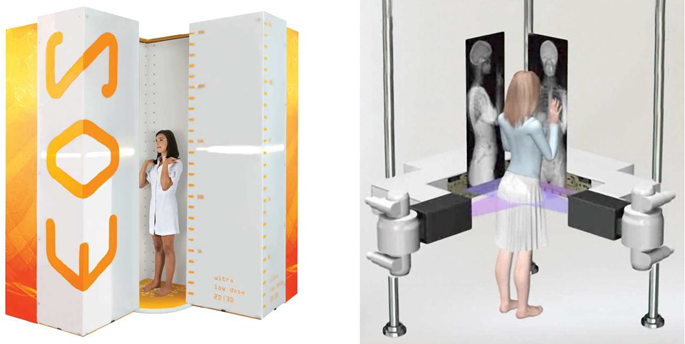
\includegraphics[width=\linewidth]{images_01/fig_01}

\textit{Vues extérieure et intérieure du système.}
\end{center}
\end{minipage}

Comme le montre la figure suivante, le bras supporte deux chaînes d’acquisition, chacune d’entre elles étant composée d’un tube à rayons X et d’un détecteur. Les tubes émettent des rayons X en pinceaux très fins qui sont ensuite recueillis par les deux détecteurs issus de la technologie ayant valu le prix Nobel de Physique à Georges Charpak en 1992.

\begin{center}
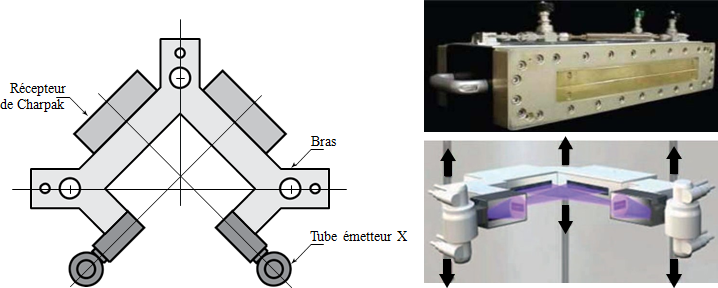
\includegraphics[width=.8\linewidth]{images_01/fig_02}

\textit{À gauche : bras mobile  vue de dessus. En haut à droite : un des deux détecteurs de Charpak. En bas à droite : émission et réception des rayons.}
\end{center}




Durant un balayage vertical de quelques secondes, les deux chaînes permettent de faire l’acquisition simultanée d’une image de face et d’une de profil du corps entier ou d’une zone anatomique choisie. À partir de ces images, un logiciel dédié permet de réaliser une modélisation tridimensionnelle du squelette du patient qui sera utilisée à des fins thérapeutiques.

On observe sur la schématisation présente que le système est constitué d’un bras mobile, guidé par rapport au bâti par trois colonnes verticales. La motorisation est assurée par trois chaînes de transmission constituées :
\begin{itemize}
\item d’un moteur électrique à courant continu commandé par l’induit ;
\item d’un réducteur à engrenages ;
\item d’une vis à billes, afin de transformer le mouvement  de rotation en mouvement  de translation.
\end{itemize}
Les noms et symboles des caractéristiques des différents composants seront donnés plus loin dans le sujet dans le tableau suivant.

\begin{center}
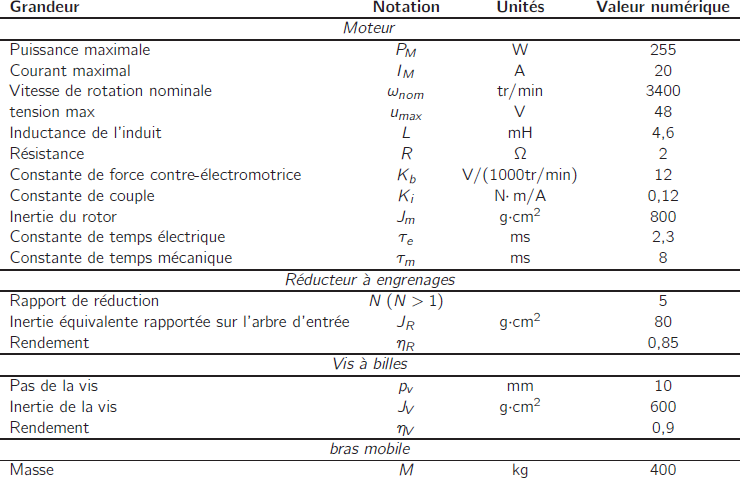
\includegraphics[width=.8\linewidth]{images_01/fig_04}
\end{center}

\subsection{Présentation}

\noindent\begin{minipage}[c]{.6\linewidth}
\begin{obj}
L’objectif de cette partie est de valider l’exigence  <<Vitesse  de déplacement  du bras>>.  Celle-ci est  primordiale  puisqu’elle impacte  directement  la qualité  des acquisitions réalisées à l’aide du système. 
\end{obj}
%Les critères associés à cette exigence sont : un écart statique nul en régulation de vitesse et une insensibilité aux perturbations en régime permanent. Cette partie s’intéresse à deux aspects de cette problématique. L’objectif du premier est de construire un modèle équivalent le plus simple possible de l’ensemble de la motorisation constituée des trois chaînes de transmission de puissance. L’objectif du deuxième est de réaliser un asservissement apte à valider les critères de précision et temps de réponse.
\end{minipage}\hfill
\begin{minipage}[c]{.35\linewidth}
\begin{center}
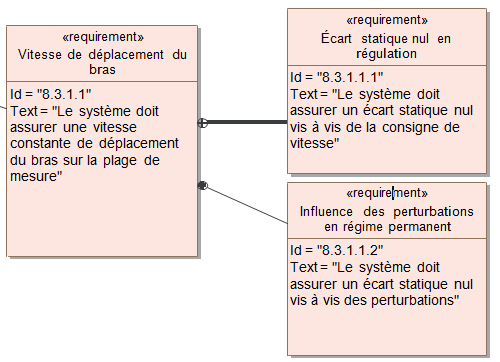
\includegraphics[width=\linewidth]{images_01/fig_03}
\end{center}
\end{minipage}

\subsection{Détermination d’un modèle dynamique de la transmission}

L’objectif est de déterminer un modèle simplifié de la motorisation complète comportant les trois chaînes de transmission de puissance. Pour cela, on déterminera  dans un premier temps  le modèle dynamique d’une transmission  ne comportant  qu’un seul moteur.  Puis on déterminera  le modèle dynamique équivalent  d’une transmission comportant 2 moteurs. Et enfin, par extension, on déterminera celui de la motorisation complète. On analysera  les caractéristiques  du modèle  obtenu afin de déterminer  si celui-ci  peut être  simplifié  en une fonction  de transfert  du premier ordre (ce  qui est  le  cas dans de nombreuses applications  comportant  des moteurs électriques à courant continu). 
%Les moteurs électriques ont été validés dans la partie précédente vis-à-vis du critère de puissance maximale à fournir. Le rendement global de la transmission étant élevé, on le prendra égal à 1 dans toute  cette  partie.


\subsubsection{Modélisation d’une motorisation ne comportant qu’un moteur}

On considère dans cette partie que le bras mobile 1 n’est entraîné en translation par rapport au bâti 0 que par une seule chaîne de transmission de puissance.% (Figure 17).

\begin{center}
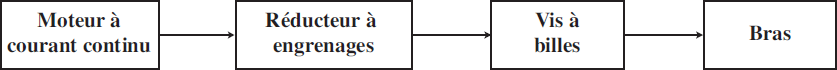
\includegraphics[width=.8\linewidth]{images_01/fig_05}
\end{center}

Le moteur à courant continu est modélisé d’un point de vue électrique par la mise en série d’une bobine équivalente d’inductance $L$, d’une résistance équivalente de résistance $R$ et d’une source de tension représentant la force contre-électromotrice $e_b$.%  (Figure 18).

%\begin{center}
%\includegraphics[width=\linewidth]{images/fig_}
%\end{center}

Les équations suivantes décrivent le comportement électrique du modèle proposé pour le moteur à courant continu :

\noindent
\begin{minipage}{.48\linewidth}
$u_m(t)=L\dfrac{\text{d}i(t)}{\text{d}t}+Ri(t)+e_b(t)$ 

$C_{meq}(t)=K_i i(t)$ 

$e_b(t)=K_b\omega_m(t)$
\end{minipage} \hfill
\begin{minipage}{.48\linewidth}
\begin{itemize} 
\item $u_m$ : tension d'alimentation du moteur;
\item $i$ : courant d’induit;
\item $e_b$ : force contre-électromotrice;
\item $C_{meq}$ : couple moteur;
\item $\omega_m$ : vitesse de rotation de l’arbre moteur.
\end{itemize}
\end{minipage}


Par ailleurs, le théorème de l'énergie cinétique appliqué  à l’ensemble E = \{bras 1, rotor du moteur, vis 3, réducteur\} permet d'écrire que :
$$
J_{eq}\dfrac{\text{d}\omega_m(t)}{\text{d} t}=C_{\text{meq}}(t)+C_{\text{Req}}(t).
$$

\subparagraph{}
\textit{Appliquer la transformée de Laplace aux équations précédentes en supposant que les conditions
initiales sont nulles et compléter le schéma-bloc. Puis, déterminer
les fonctions de transfert $H_m(p)$ et $H_C(p)$ associées aux deux entrées $U_m(p)$ et $C_{\text{req}}(p)$ de telle sorte
que :}

$$
\Omega_m(p)=H_m(p)U_m(p)+H_c(p)C_{\text{req}}(p).
$$

Il n’est pas utile à ce stade de l’étude de déterminer  la forme canonique des fonctions de transfert, mais une écriture sous la forme $\dfrac{N(p)}{D(p)}$  (où $N(p)$ et $D(p)$ sont deux polynômes) est attendue.

\subsubsection{Modélisation d’une motorisation comportant deux chaînes de transmission}
Nous allons dans cette partie décrire le comportement obtenu avec l’association de deux chaînes de transmission en parallèle.

\begin{center}
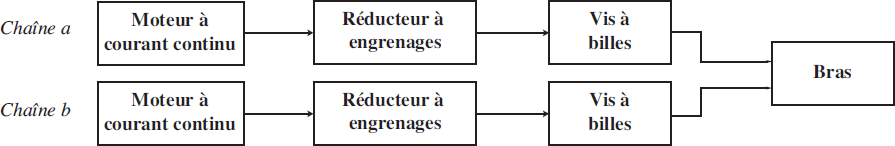
\includegraphics[width=\linewidth]{images_01/fig_06}
\textit{Motorisation comportant deux chaînes de transmission de puissance.}
\end{center}

On considère les équations suivantes décrivant le comportement dynamique  des deux chaînes. Les indices $a$ et $b$ évoquent respectivement les moteurs des chaînes $a$ et $b$.

\noindent
\begin{minipage}{.48\linewidth}
Les équations concernant le moteur $a$ sont :
$$  (1) \left\{
\begin{array}{l}
u_{ma}(t)=L_a\dfrac{\text{d}i_a(t)}{\text{d}t}+R_ai_a(t)+e_{ba}(t) \\

C_{ma}(t)=K_{ia} i_a(t) \\

e_{ba}(t)=K_{ba} \omega_m(t) \\
\end{array}
\right.
$$
\end{minipage} \hfill
\begin{minipage}{.48\linewidth}
Les équations concernant le moteur $b$ sont :
$$ (2) \left\{
\begin{array}{l}
u_{mb}(t)=L_b\dfrac{\text{d}i_b(t)}{\text{d}t}+R_bi_b(t)+e_{bb}(t) \\

C_{mb}(t)=K_{ib} i_b(t) \\

e_{bb}(t)=K_{bb} \omega_m(t) \\
\end{array}
\right.
$$

\end{minipage}

Les deux chaînes de transmission étant reliées au même bras mobile 1 en translation par rapport au bâti, les deux moteurs tournent à la même vitesse. L’équation traduisant le comportement mécanique est alors :
$$
(3)  \quad
J_{eq2}\dfrac{\text{d}\omega_m(t)}{\text{d} t}=C_{\text{ma}}(t)+C_{\text{mb}}(t)+C_{\text{Req2}}(t).
$$

\subparagraph{}\textit{Appliquer la transformée de Laplace aux équations (1), (2) et (3) en supposant que les conditions initiales sont nulles et compléter le schéma-blocs.}

\subparagraph{}
\textit{En considérant que les deux moteurs sont identiques ($L_a  = L_b$ , $R_a = R_b$, ...), déterminer les fonctions de transfert $H_{ma}$, $H_{mb}$ et $H_{C2}$ associées aux trois entrées $U_{ma}$ , $U_{ma}$ et $C_{\text{Req2}}$ de telle sorte que :}
$$\Omega_m (p) = H_{ma}(p) U_{ma}(p) + H_{mb} (p) U_{mb} (p) + H_{C2}(p) C_{\text{Req2}} (p).$$

Il n’est pas utile  à ce stade de l’étude de déterminer la forme canonique des fonctions de transfert, mais une écriture sous la forme (où $N(p)$ et $D(p)$ sont deux polynômes) est attendue.


\subparagraph{}
\textit{En considérant  que les 2 moteurs  sont alimentés  par la même  tension  $u_m(t)$ , montrer, dans un premier temps, que l’équation précédente peut se mettre  sous la forme de l’équation  suivante correspondant à une motorisation comportant un unique moteur équivalent, puis déterminer les caractéristiques équivalentes $K_{i 2}$ , $K_{b 2}$ , $J_{eq2}$ , $R_2$, $L_2$  de ce moteur équivalent?}
$$
\Omega_m(p)=H_{eq2m}(p)U_m(p)+H_{Ceq2m}(p)C_{Req2}(p)
$$

\subsubsection{Modélisation et analyse du comportement de la motorisation complète}

On considère dans cette partie la motorisation comportant les trois chaînes de transmission de puissance.

\begin{center}
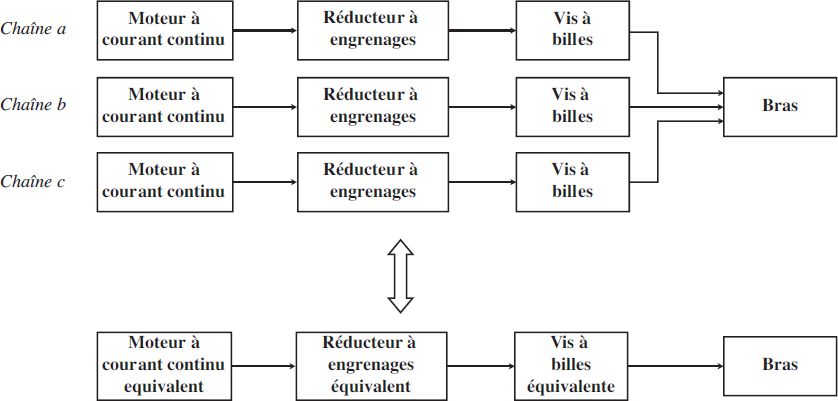
\includegraphics[width=.7\linewidth]{images_01/fig_07}

\textit{Chaîne de motorisation équivalente.}
\end{center}

\subparagraph{}
\textit{En utilisant les résultats obtenus à la question précédente, donner par analogie les expressions des coefficients  $K_{i 3}$, $K_{b3}$, $J_{eq3}$, $R_3$, $L_3$  de la motorisation équivalente ne comportant qu’une seule chaîne (moteur, réducteur, liaison hélicoïdale) correspondant à l’équation suivante :}
$$
\Omega_m(p)=H_{eq3m}(p)U_m(p)+H_{Ceq3m}(p)C_{Req3}(p)
$$

\subparagraph{}
\textit{Déterminer les formes canoniques des fonctions de transfert $H_{eq3m}(p)$ et $H_{Ceq3m}(p)$ et donner les expressions des termes $a$, $b$, $K_m$ , $K_C$ , $\tau_C$  tels que :}

$H_{eq3m}(p)=K_m\dfrac{1}{ap^2+bp+1}$ et $H_{Ceq3m}(p)=K_C\dfrac{1+\tau_c p}{ap^2+bp+1}$.



\subparagraph{}
\textit{Déterminer la valeur numérique de $K_{b3}$  en $\text{V.s.rad}^{-1}$.}

\subparagraph{}
\textit{Déterminer la valeur numérique de $J_{eq3}$ en $\text{kg m}^2$. Quelle est, en pourcent, la proportion provenant de la totalité des inerties des trois réducteurs, des trois vis et de la masse du bras
dans cette valeur.}

\subparagraph{}
\textit{À partir des valeurs numériques du tableau donné précédemment, montrer que l’on peut factoriser le
dénominateur de $H_{eq3m}$ sur le corps des réels. Déterminer alors les expressions des constantes de temps $\tau_1$ et $\tau_2$ telles que :
$ap^2 + bp + 1 = (1 + \tau_1p)(1 + \tau_2 p)$. 
Une résolution numérique donne : $\tau_1 \simeq \SI{0,0025}{s}$ et $\tau_2 \simeq \SI{0,012}{s}$. Peut-on considérer l’un des modes comme dominant ?}

\subsection{Asservissement et détermination du correcteur}
Les calculs suivants sont menés en considérant le modèle équivalent qui vient d’être déterminé. À  partir de ce point, quels que soient les résultats obtenus précédemment, on conservera  les notations $K_m$, $K_C$, $\tau_1$, $\tau_2$ et $\tau_C$  pour les caractéristiques des fonctions de transfert du modèle équivalent aux trois chaînes de transmission de puissance. On prendra donc :
$$
H_{eq3m}(p)=\dfrac{K_m}{\left(1+\tau_1 p\right)\left(1+\tau_2 p\right)} 
\quad
\text{et}
\quad
H_{Ceq3m}(p)=\dfrac{K_C\left(1+\tau_C p\right)}{\left(1+\tau_1 p\right)\left(1+\tau_2 p\right)} 
$$
avec $K_m  = \SI{8}{rad.s^{-1}.V^{-1}}$, $\tau_1\simeq \SI{0,0025}{s}$  et $\tau_2  \simeq \SI{0,012}{s}$. Les valeurs numériques de $K_C$  et $\tau_C$  ne sont pas utiles pour les problématiques abordées dans cette partie.

Pour répondre  au cahier  des charges défini par le tableau suivant, on réalise  un asservissement de la vitesse de rotation des vis. Le schéma-blocs correspondant est celui donné ci-après, avec les grandeurs physiques suivantes :
\begin{itemize}
\item $v_c (t)$ : vitesse de consigne du bras mobile 1 ;
\item $u_c (t)$ : tension de consigne ;
\item $\varepsilon(t)$ : écart en tension ;
\item $\Omega_v (t)$ : vitesse de rotation d’une vis $3_k$;
\item $v(t)$ : vitesse du bras mobile 1 ;
\item $m(t)$ : mesure de la vitesse de rotation d’une vis $3_k$.
\end{itemize}



\begin{center}
\begin{tabular}{|p{6cm}|p{2cm}|p{2cm}|}
\hline
Critère & Valeur & Variabilité \\
\hline
\hline 
Temps de réponse à 5\% & \SI{0,75}{s}& max \\ \hline
Marge de phase & \SI{65}{\degres}& min\\ \hline
Marge de gain & \SI{8}{dB}& min\\ \hline
Écart statique en régulation& \SI{0}{ms^{-1}}&\\ 
\hline
\end{tabular}
\end{center}


\begin{center}
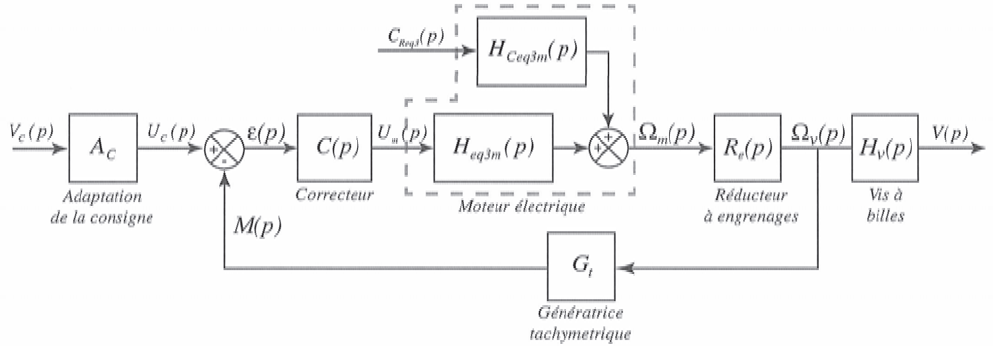
\includegraphics[width=\linewidth]{images_01/fig_08}
\textit{Schéma d'asservissement de la vitesse des vis $3_k$.}
\end{center}

Le capteur est une génératrice tachymétrique fixée sur l’axe de rotation d’une des trois vis. On considérera que la dynamique de ce capteur est très grande par rapport aux constantes de temps de la chaîne directe. Sa fonction de transfert sera donc modélisée par un gain pur $G_t  = \SI{0,1}{V.rad^{-1} s}$.



\subparagraph{}
\textit{Donner les expressions des fonctions de transfert $R_e (p)$  et  $H_v (p)$  en  fonction  des  caractéristiques des réducteurs et de la vis du tableau page 2.}

\subparagraph{}
\textit{Quelle doit être la valeur numérique du gain $A_C$ pour que l'écart de tension $\varepsilon(t)$ ait un sens ?}


\subparagraph{}
\textit{Expliquer pourquoi il n’est pas possible de vérifier toutes les exigences du cahier des charges en utilisant un correcteur proportionnel.}

On choisit un correcteur de type intégrateur : $C(p)=\dfrac{K_{cor}}{p}$.


\subparagraph{}
\textit{Déterminer la fonction de transfert en boucle ouverte $FTBO(p)$ telle que : $M(p)=FTBO(p)\varepsilon(p)$.}



\subparagraph{}
\textit{On donne sur le document réponse le diagramme de Bode de la phase de la fonction de transfert $\text{FTBO}(p)$. En considérant $K_{\text{Cor}}$ unitaire,  tracer le diagramme  de Bode asymptotique du gain de $\text{FTBO(p)}$.}


\subparagraph{}
\textit{Par analogie  avec  un système  du premier  ordre  de temps  de réponse  $T_{R5\%}   =\SI{0,75}{s}$, déterminer  la valeur de la pulsation  à  $\SI{0}{dB}$ souhaitée.  Déterminer  la valeur minimale  du gain $K_{\text{Cor}}$ qui permet de respecter ce critère. Quelles sont alors les marges de phase et de gain ?}


\subsection{Validation du système de commande}

Afin de valider le système de commande, il est nécessaire de réaliser dans un premier temps des simulations des évolutions dans le domaine temporel de certaines grandeurs physiques. Pour réaliser cette simulation, il est nécessaire d’introduire la valeur numérique du couple résistant équivalent rapporté sur l’arbre moteur.

\subparagraph{}
\textit{Déterminer la valeur numérique du couple résistant $C_{\text{Req3}}$ rapporté sur l’arbre moteur.}
\vspace{.25cm}

Une simulation a permis d’obtenir  les évolutions temporelles  de la vitesse et de la position du bras 1, de la tension d’alimentation d’un moteur et de l’intensité du courant le traversant, en réponse à une consigne en
vitesse de $\SI{10}{cm.s^{-1}}$ et d’un couple résistant constant déterminé à la question précédente

\begin{center}
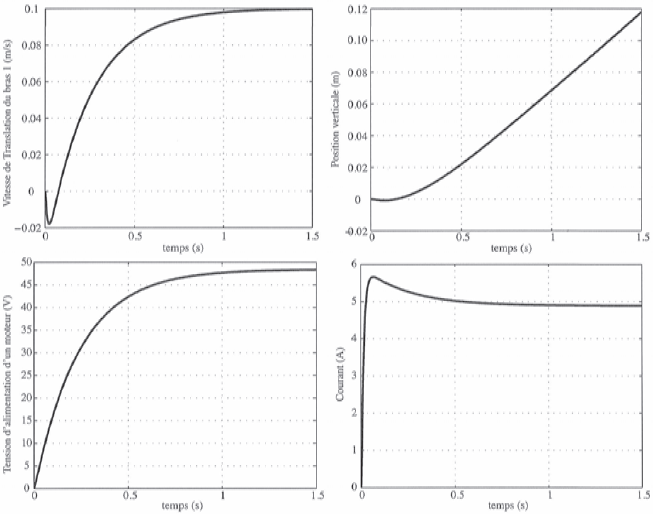
\includegraphics[width=\linewidth]{images_01/fig_09}
\textit{Évolutions temporelles  de la vitesse et de la position du bras 1 (en haut), de la tension d’alimentation d’un moteur et de l’intensité du courant le traversant (en bas).}
\end{center}

\subparagraph{}
\textit{Valider les différents éléments du cahier des charges ainsi que les caractéristiques limites du moteur précisées dans le tableau de la page 2.
}

\subparagraph{}
\textit{Expliquer, en 5 lignes maximum,  la forme de la courbe donnant l’évolution de la vitesse du bras 1 en fonction du temps au voisinage de 0. Quel élément sur le système réel faut-il prévoir afin d’éviter ce comportement ?}

\newpage

\section{Banc d'épreuve hydraulique}
\subsection{Présentation}
Vallourec \& Mannesmann Tubes (V\&M Tubes), entreprise du groupe Vallourec, est le leader mondial dans la production de tubes en acier sans soudure laminés à chaud. L’entreprise exploite des tuberies équipées des installations les plus modernes : quatre en France, quatre en Allemagne, trois  aux USA et au Brésil et une ligne de finition en Chine.
Les tubes sans soudure en acier produits par V\&M Tubes couvrent une très large gamme tant sur le plan dimensionnel que dans la nature des matériaux.
% :
%•	les diamètres extérieurs vont de 21,3 mm à 1,5 m, les épaisseurs de 2 à 250 mm ;
%•	outre les aciers non alliés et alliés, V&M Tubes produit des tubes en aciers spéciaux élaborés pour s’adapter aux applications spécifiques des clients.
%Ces tubes sont employés dans des applications très diverses : 
%•	canalisations hydrauliques, pneumatiques, vapeur ;
%•	ventilation, climatisation ;
%•	en basse pression ou haute pression…
%Les industries utilisatrices sont tout aussi variées. Pour certaines d’entre elles, telles que les industries pétrolières ou nucléaires par exemple, où les problèmes de sécurité sont particulièrement importants, il arrive que les clients exigent des qualités spécifiques pour leurs tubes en plus des critères liés au cahier des charges standard. Une de ces contraintes personnalisées est la garantie de la tenue des tubes à un seuil de pression durant un temps donné.
Le site de V\&M Tubes situé à Aulnoye-Aymeries, qui produit des tubes de 114 mm à 508 mm de diamètre pour des longueurs variant de 4,40 à 14,20 m possède un banc spécifique de test de pression hydraulique pour valider la qualité des produits finis exigée par certains clients. C’est le fonctionnement de ce banc conçu par M\&T Tubes qui fait l’objet de cette étude.

Afin de valider la caractéristique de tenue en pression des tubes, ceux-ci sont soumis à une pression hydraulique donnée durant un temps spécifié. Ces paramètres dépendent de la taille des tubes et de leur future utilisation.

\subsection{Analyse de la fonction technique << mettre le tube sous pression >>.}

La finalité de la mise sous pression est de vérifier la résistance du tube pour une pression maximale imposée par le client. Le cahier des charges impose un écart statique en pression inférieur à 5\% et aucun dépassement. 
Les objectifs de cette partie sont de modéliser le système de mise sous pression afin de vérifier le respect de ce cahier des charges et au besoin de proposer des modifications de la commande pour pallier les écarts observés.

Un schéma hydraulique simplifié est donné figure suivante :
\begin{center}
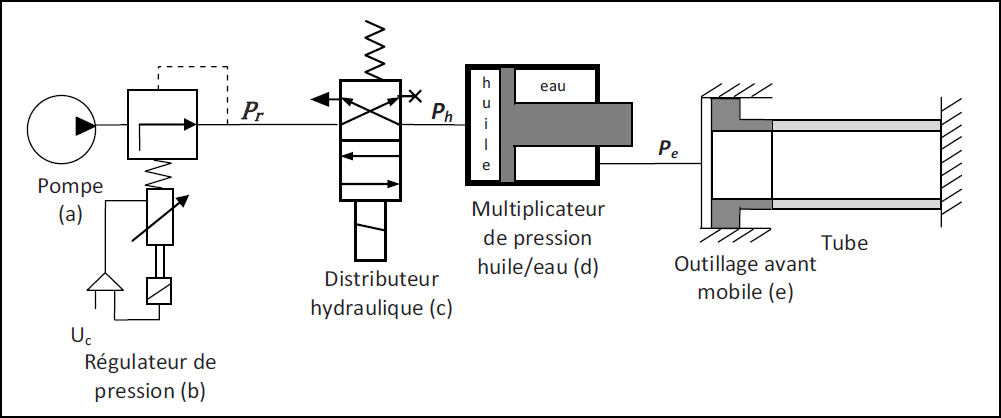
\includegraphics[width=\linewidth]{images_02/fig_01}
%\textit{Schéma d'asservissement de la vitesse des vis $3_k$.}
\end{center}


\begin{itemize}
\item Le fluide injecté dans le tube est de l’eau sous pression.
\item Dans un premier temps, l’opérateur règle la tension consigne Uc de mise sous pression par l’intermédiaire d’un potentiomètre (non représenté), une plage de tension de 0 à \SI{2,5}{V} correspondant à une consigne de pression d’eau comprise entre 0 et \SI{1000}{bars}.
\item La pompe (a) fournit de l’huile dont la pression est réglée par un régulateur de pression (b) piloté par cette tension consigne $U_c$.
\item Un distributeur hydraulique (c) pilote la montée d’un multiplicateur de pression huile/eau (d) ;
Ph désigne la pression d’huile en entrée et $P_e$ la  pression d’eau en sortie.
\item L’eau est injectée par l’outillage avant (e) dans le tube. Sa pression est mesurée par un capteur de pression de gain $K_{cap} = 2,5\cdot 10^{-3} \text{V/bars}$  (non représenté).
\end{itemize}

\subsubsection{Mise en place du modèle}

Jusqu’à la Question 24, on négligera le temps de réponse de cet ensemble face à la dynamique du distributeur, du multiplicateur de pression et de l’outillage avant de mise sous pression. On supposera donc que la pression en sortie du régulateur est constante, égale à $P_r$.

Le distributeur hydraulique fournit un débit d’huile défini par l’équation : 
	$Q_h (t)=K_r.\sqrt{P_r (t)-P_h (t)}$, avec $K_r$ constante en $\text{m}^3.\text{Pa}^{-1/2}$, avec :
\begin{itemize}
\item $P_r(t)$ : pression en entrée du distributeur (sortie du régulateur);
\item $P_h(t)$ : pression en sortie du distributeur.
\end{itemize}


\begin{minipage}[c]{.65\linewidth}
Le multiplicateur, représenté ci-contre, se compose d’un piston, de masse $M$, en translation par rapport au bâti, séparant les chambres $C_e$ et $C_h$ comportant respectivement de l’eau et de l’huile sous pression.
On note :
\begin{itemize}
\item $Q_e(t)$ : le débit volumique d’eau en sortie du multiplicateur;
\item $Q_h(t)$ : le débit volumique d’huile en entrée du multiplicateur;
\item $P_e(t)$ : la pression d’eau dans $C_e$;
\item $P_h(t)$ : la pression d’huile dans $C_h$;
\item $z(t)$ : la position du piston;
\item $V_e(t)$ : le volume de $C_e$;
\item $V_h(t)$ : le volume de $C_h$;
\item $g$ : l’accélération de pesanteur;
\item $\vect{z}$ : le vecteur vertical unitaire ascendant.
\end{itemize}

Les équations du débit sont : 
$$
	Q_e (t)=S_e\dfrac{\text{d}z(t)}{\text{d}t}-\dfrac{V_{e0}}{B_e}   \dfrac{\text{d}P_e (t)}{\text{d}t}
\quad
	Q_h (t)=S_h\dfrac{\text{d}z(t)}{\text{d}t}+\dfrac{V_{h0}}{B_h}   \dfrac{\text{d}P_h (t)}{\text{d}t}
$$
\end{minipage}\hfill
\begin{minipage}[c]{.3\linewidth}
\begin{center}
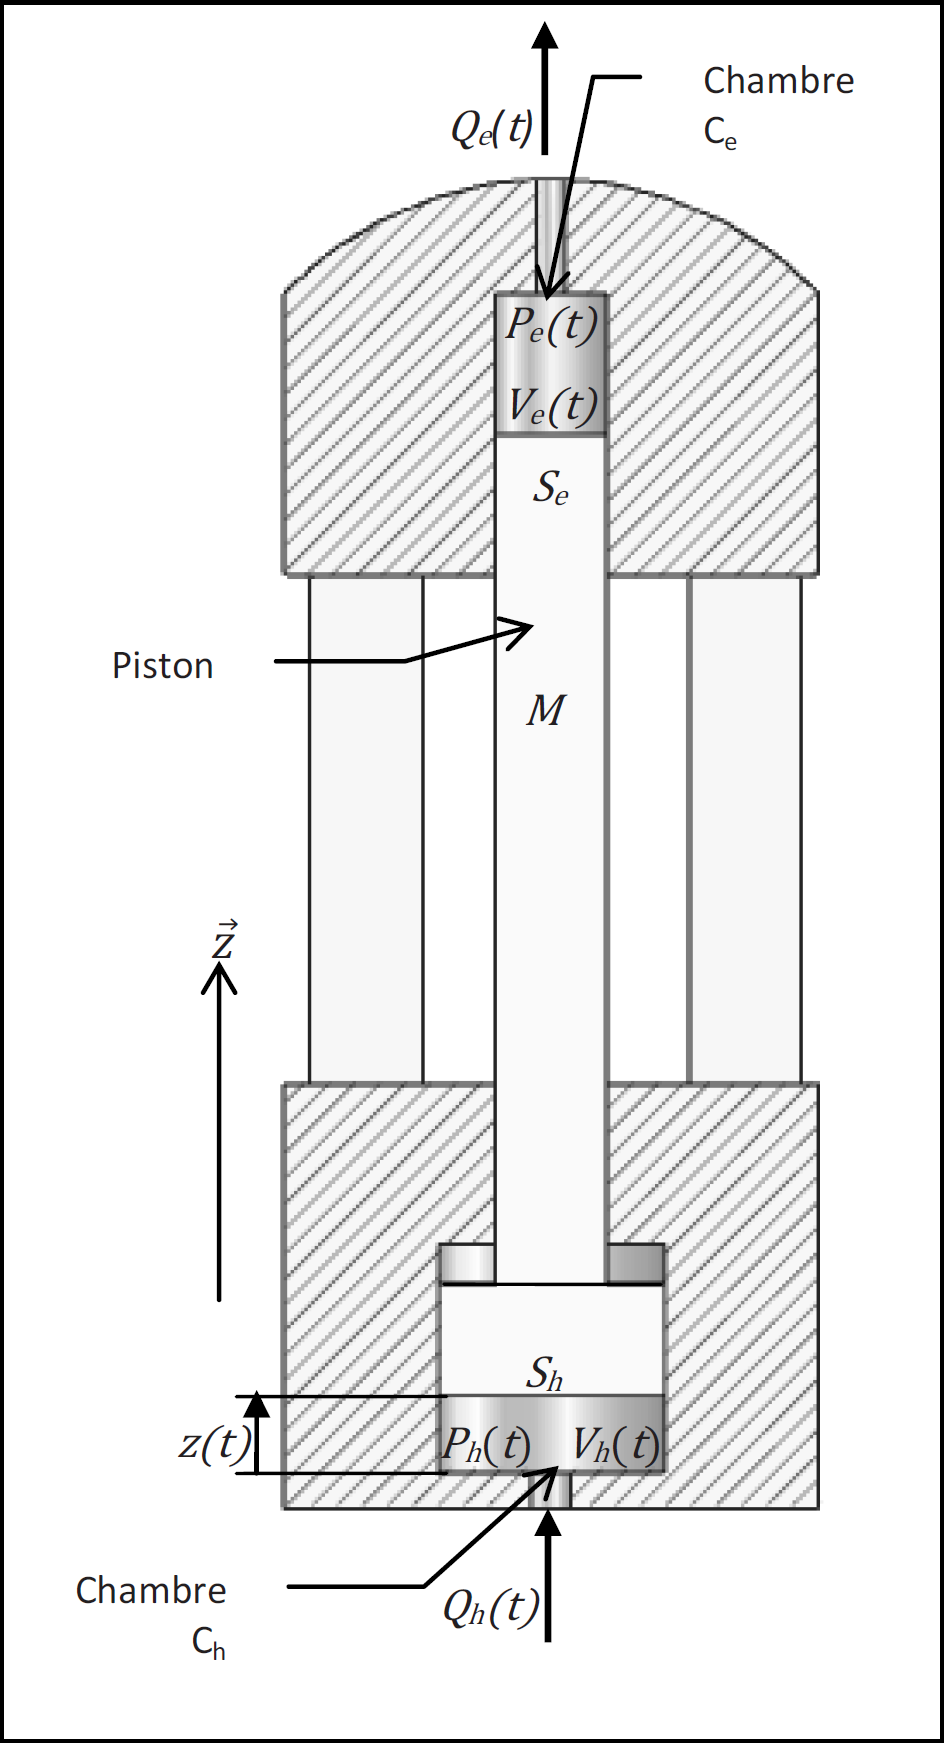
\includegraphics[width=\linewidth]{images_02/fig_02}
%\textit{Schéma d'asservissement de la vitesse des vis $3_k$.}
\end{center}
\end{minipage}

Données numériques : 
\begin{multicols}{2}
\begin{itemize}
\item $S_e$ :	section du piston dans la chambre $C_e = \SI{397,6}{10^{-4}m^2}$;
\item $S_h$ :	section du piston dans la chambre $C_h = \SI{1288,25}{10^{-4}m^2}$;
\item $B_e$ :	module de compressibilité de l’eau = \SI{2.109}{Pa};
\item $B_h$ :	module de compressibilité de l’huile = \SI{109}{Pa};
\item $M$ :	masse du piston = \SI{668}{kg};
\item $f$ :	coefficient de frottement visqueux = $10^6 \, \text{N/m/s}$;
\item $V_{e0}$ :	volume initial de la chambre $C_e =  1,2.10^{-2}\,\text{m}^3$;
\item $V_{h0}$ :	volume initial de la chambre $C_h = 3,8.10^{-2}\,\text{m}^3$.
\end{itemize}
\end{multicols}
En appliquant le théorème de la résultante dynamique selon $\vect{z}$ sur le piston du multiplicateur, on a : 
$$
M\ddot{z}(t)=S_hp_h(t)-S_ep_e(t)-Mg-f\dot{z}(t).
$$
\subparagraph{}
\textit{Déduire de la relation précédente l’équation reliant $Z(p)$, $P_e(p)$, $P_h(p)$, et $\text{Poids}(p)=Mg/p$, transformées de Laplace de $z(t)$, $P_e(t)$, $P_h(t)$ et du poids perçu comme une perturbation. Les conditions initiales sont supposées nulles.}

\subsubsection{Modélisation du chariot avant}
Le chariot avant comporte :
\begin{itemize}
\item la traverse, mise en position par un vérin hydraulique avant la mise sous pression du tube. Durant toute la durée de l’épreuve, on supposera que la traverse est immobile par rapport au bâti;
\item un équipage mobile sur lequel est monté l’outillage, en translation rectiligne par rapport à la traverse.
\end{itemize}



\begin{center}
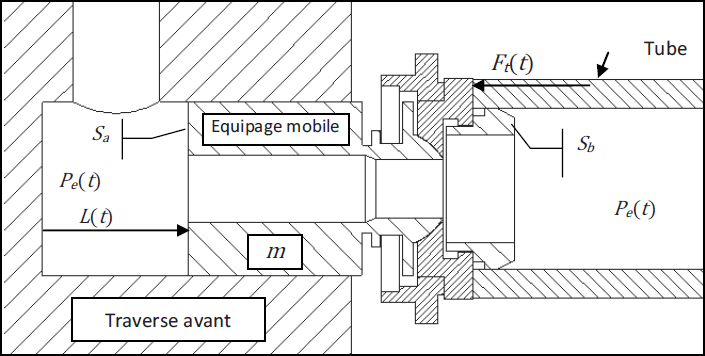
\includegraphics[width=.8\linewidth]{images_02/fig_03}
%\textit{Schéma d'asservissement de la vitesse des vis $3_k$.}
\end{center}


On note :
\begin{itemize}
	\item $L(t)$ la position de l’équipage mobile repérée par rapport à sa position initiale;
	\item $V_t(t)$ le volume du tube;
	\item $F_t(t)$ l’effort du tube sur l’équipage mobile, avec $F_t(t) = - rL(t)$.
\end{itemize}

On néglige les variations de volume du tube dues à ses déformations. L’équation du débit s’écrit alors :
	$$Q_e (t)=(S_a-S_b ).\dfrac{\text{d}L(t)}{\text{d}t}+\dfrac{V_t}{B_e}  \dfrac{\text{d}P_e (t)}{\text{d}t}.$$
	
	
Données numériques :
\begin{itemize}
	\item $S_a$ et $S_b$ :	sections de l’équipage mobile côté tube et côté opposé au tube,
$S_a -S_b  = \SI{1,88}{10^{-3}.m^2}$;	
	\item $m$ :		masse de l’ensemble mobile = \SI{25}{kg};
	\item $f ’$ :		coefficient de frottement visqueux = 10 N/(m/s);
	\item $V_t$ :		le volume du tube = \SI{1,34}{m^3};
	\item $r$ :		le tube est assimilé à un ressort de raideur = \SI{5}{10^8.N/m}.
\end{itemize}

%\begin{center}
%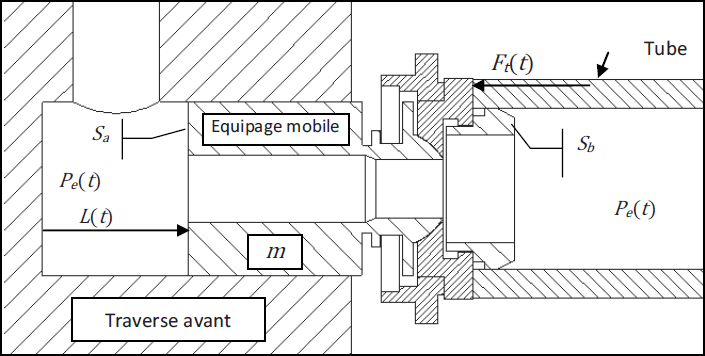
\includegraphics[width=\linewidth]{images_02/fig_03}
%\end{center}

L’équation du mouvement de l’équipage mobile est donnée par : 
$$
m\ddot{L}(t)=-rL(t)+\left(S_a-S_b \right)p_e(t)-f'\dot{L}(t).
$$

\subparagraph{}
\textit{En déduire, en tenant compte de l’équation du débit, deux équations liant $L(p)$, $P_e(p)$ et $Q_e(p)$, transformées de Laplace de $L(t)$, $P_e(t)$ et $Q_e(t)$. }

Les conditions initiales sont supposées nulles.

\subparagraph{}
\textit{Sur le document réponse, compléter le schéma bloc de l’ensemble (sans le distributeur hydraulique), l’entrée étant la pression d’huile régulée $P_r(p)$ et la sortie la pression d’épreuve dans le tube $P_e(p)$.}



La figure suivante représente la réponse de l’ensemble de mise sous pression pour un échelon de 250 bars : $P_r$ est la pression d’huile en sortie du régulateur, $P_h$ la pression d’huile dans le distributeur et $P_e$ la pression d’eau dans le tube.

\begin{center}
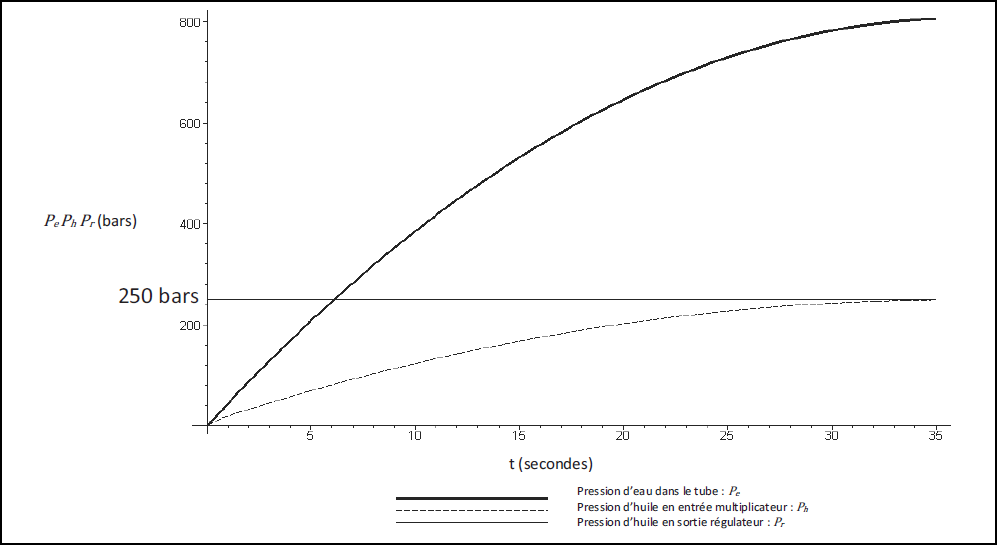
\includegraphics[width=\linewidth]{images_02/fig_04}
\end{center}

\subparagraph{}
\textit{À partir de ces réponses temporelles, proposer une expression numérique des fonctions de transfert $P_h(p)/P_r(p)$, $P_e(p)/P_r(p)$. Justifier vos valeurs numériques.}

\vspace{.25cm}

De nombreuses fuites au niveau de l’outillage avant influent sur la réponse. À cause de ces fuites, le débit d’eau en entrée du tube est $Q’_e(t) = Q_e(t)-\Delta Q_e$, $\Delta Q_e$ étant le débit de fuite, supposé constant.
La suivante représente la réponse de l’ensemble de mise sous pression à un échelon de 250 bars avec fuite d’eau à partir de \SI{35}{s}. Le débit de fuite est supposé pour cette étude, égal à $\Delta Q_e = \SI{2}{10^{-3}.m^3/s}$.

\begin{center}
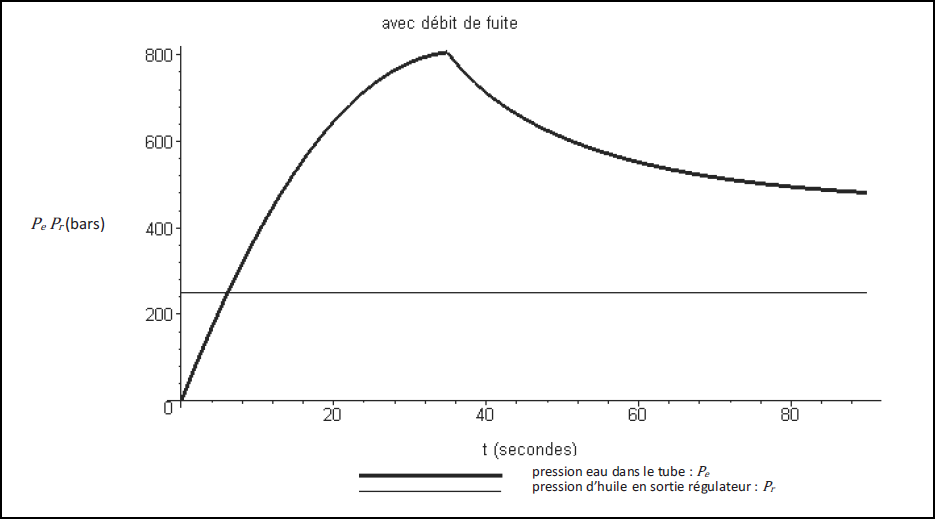
\includegraphics[width=\linewidth]{images_02/fig_05}
\end{center}

\subparagraph{}
\textit{À partir de ces réponses temporelles, proposer une expression numérique de la fonction de transfert en régulation $\dfrac{P_e(p)}{\Delta Q_e(p)}$.}

\subsection{Mise en place d'un asservissement de pression.}
Pour limiter l’erreur statique due aux fuites, on envisage d’asservir la pression d’eau dans le tube. L’objectif est ici de proposer un réglage du correcteur pour répondre aux critères du cahier des charges.
La pression d’eau à l’intérieur du tube est mesurée par un capteur de pression. Le schéma-blocs de l’asservissement est défini ci-dessous.

\begin{center}
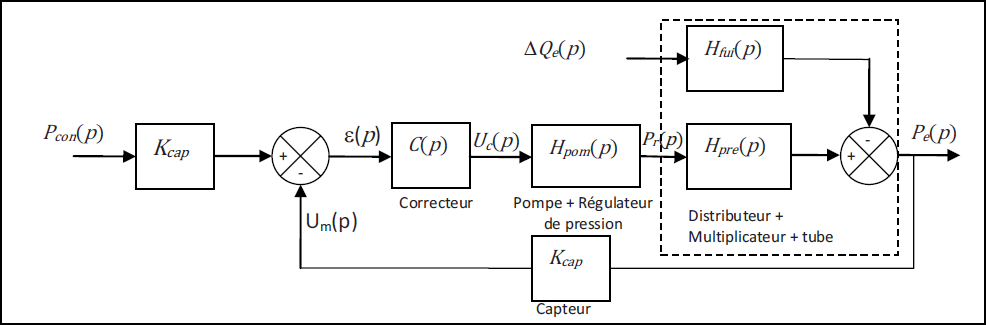
\includegraphics[width=\linewidth]{images_02/fig_06}
\end{center}

\begin{itemize}
\item $P_{con}(p)$ 	: 	pression de consigne d’eau dans le tube (Pa);
\item $P_e(p)$ 	:	pression d’eau dans le tube (Pa);
\item $U_c(p)$ 	: 	tension de commande du régulateur de pression (V);
\item $P_r(p)$ 	:	pression d’huile régulée (Pa);
\item $\Delta Q_e(p)$ 	:	débit de fuite ($\text{m}^3/\text{s}$);
\item $U_m(p)$ 	:	tension de mesure du capteur (V).
\end{itemize}

Hypothèses : 
\begin{itemize}
\item quels que soient les résultats précédents, l’ensemble de mise sous pression \{tube + distributeur + multiplicateur de pression\} est défini par les transmittances suivantes :
$H_{pre} (p)=\dfrac{K_m}{1+T_1 p}$ et $H_{fui} (p)=\dfrac{K_f}{1+T_1 p}$
avec $K_m = 3,24$; $K_f = \SI{2,55}{10^{10} Pa/(m^3/s)}$; $T_1  =\SI{10}{s}$; 
\item l’ensemble \{pompe+régulateur de pression\} est modélisé par la fonction de transfert :
$H_{pom} (p)=\dfrac{K_{pom}}{1+T_2 p}$ avec $K_{pom} = \SI{1,234}{10^7 Pa/V}$; 	$T_2 = \SI{5}{s}$;
\item le capteur est modélisé par un gain pur :	$K_{cap}= \SI{2,5}{10^{-8}.V/Pa}$.
\end{itemize}

La pression de consigne est de $P_{con} = \SI{800}{bars}$ et les débits de fuite sont estimés à $\Delta Q_e = \SI{5}{10^{-4} m^3/s}$.

On rappelle que le cahier des charges concernant le réglage de la pression de test est le suivant :
\begin{center}
\begin{tabular}{|l|p{10cm}|}
\hline
Stabilité : & marge de phase de $60\degres$

 marge de gain de \SI{12}{dB} \\ \hline
Rapidité :	&temps d’établissement $t_e < \SI{40}{s}$ \\ \hline
Précision :&	erreur statique < 5\% soit pour une consigne de 800 bars :

erreur statique due à la consigne : $\varepsilon_{con} < 5\%$ 

erreur statique due à la perturbation $\varepsilon_{pert} < \SI{40}{bars}$ \\ \hline

Amortissement :&	pas de dépassement \\ \hline
\end{tabular}
\end{center}

Dans le cas d’un système bouclé convenablement amorti, on pourra utiliser, sans aucune justification, la relation : 	$t_e \omega_{\SI{0}{dB}}=3$ 
où $\omega_{\SI{0}{dB}}$ désigne la pulsation de coupure à \SI{0}{dB} en boucle ouverte et $t_e$ le temps d’établissement en boucle fermée vis-à-vis d’un échelon de consigne :
\begin{itemize}
\item $t_e = t_m$, temps du 1\ier maximum si le dépassement est supérieur à 5\%;
\item $t_e = t_R$, temps de réponse à 5\% si le dépassement est nul ou inférieur à 5\%.
\end{itemize}
On envisage tout d’abord un correcteur de type proportionnel : $C(p)=K_p$. 


\subparagraph{}
\textit{Déterminer, en fonction de $K_p$ , $\varepsilon_{con}$ définie comme l’erreur statique pour une entrée consigne $P_{con}$ de type échelon, dans le cas où le débit de fuite est nul.}

\subparagraph{}
\textit{Proposer un réglage de $K_p$ pour limiter $\varepsilon_{con}$ à la valeur spécifiée dans le  cahier des charges.}

\subparagraph{}
\textit{Dans le cas où la consigne de pression est nulle,  déterminer en fonction de $K_p$ la fonction de transfert en régulation définie par :
$H_{pert} (p)=\dfrac{P_e (p)}{\Delta Q_e (p)}$.
En déduire, en fonction de $K_p$ , $\varepsilon_{pert}$ définie comme l’erreur statique pour une perturbation $\Delta Q_e$ de type échelon, dans le cas où la consigne de pression est nulle.}

\subparagraph{}
\textit{Proposer un réglage de $K_p$ pour limiter $\varepsilon_{pert}$ à la valeur spécifiée au cahier des charges.}

\subparagraph{}
\textit{Proposer un réglage de $K_p$ pour vérifier le critère d’amortissement. \'A partir des résultats des questions précédentes, conclure quant au choix d’un correcteur proportionnel.}

On se propose de corriger le système avec le correcteur défini sur le schéma-blocs ci-dessous :
\begin{center}
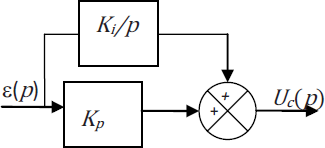
\includegraphics[width=.4\linewidth]{images_02/fig_07}
\end{center}


\subparagraph{}
\textit{Déterminer la fonction de transfert $C(p)$ de ce correcteur.}

\subparagraph{}
\textit{Tracer l’allure de son diagramme de Bode en fonction des coefficients $K_i$ et $K_p$.}

\subparagraph{}
\textit{Quelle est l’influence d’un tel correcteur sur la précision et la stabilité ? Justifier.}

\subparagraph{}
\textit{Quelle valeur faut-il donner à $\omega_{0dB}$ pour répondre au critère de rapidité du cahier des charges ?}

\subparagraph{}
\textit{Déterminer alors le rapport $T=K_p/K_i$ pour obtenir la marge de phase spécifiée dans le cahier des charges.}

\subparagraph{}
\textit{En déduire les valeurs de $K_p$ et de $K_i$ qui permettent de régler rapidité et marge de phase.}


On donne les diagrammes de Bode en gain et en phase de la fonction de transfert en boucle ouverte corrigée avec le correcteur Proportionnel Intégral déterminé précédemment.

\begin{center}
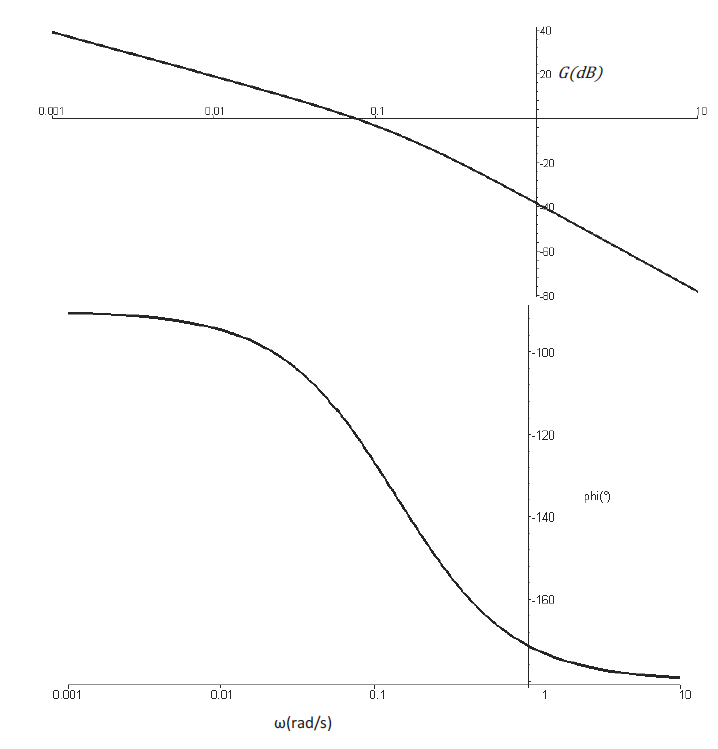
\includegraphics[width=.8\linewidth]{images_02/fig_08}
\end{center}

On donne ensuite sa réponse temporelle avec et sans débit de fuite pour une pression de consigne d’eau de 800 bars.


\begin{center}
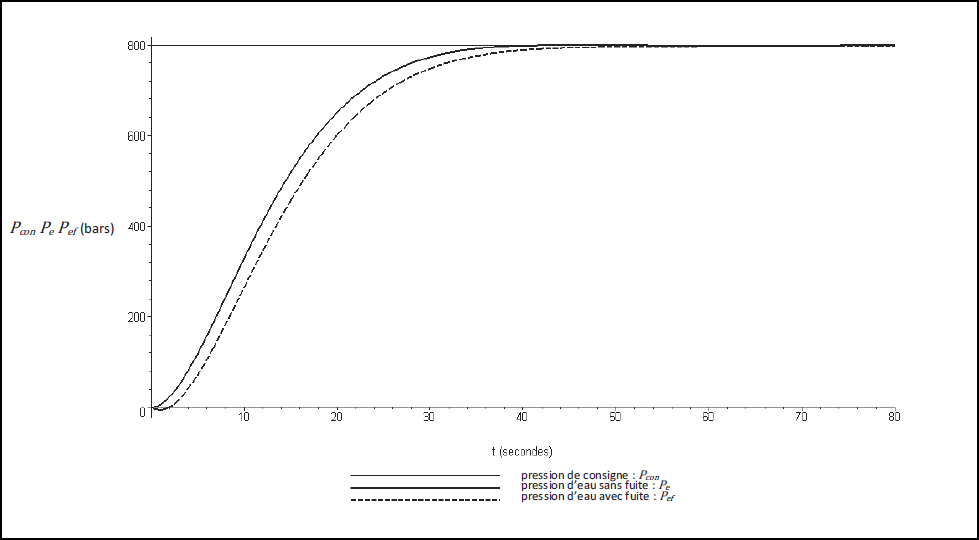
\includegraphics[width=.8\linewidth]{images_02/fig_09}
\end{center}

\subparagraph{}
\textit{La réponse du système est-elle satisfaisante au regard du cahier des charges ? Justifier.}



\end{document}

\subparagraph{}
\textit{}
\ifprof
\begin{corrige}
\end{corrige}
\else
\fi
  